\documentclass[smallabstract,smallcaptions]{dccpaper}

\usepackage{epsfig}
\usepackage{amsmath}
\usepackage{amssymb}
\usepackage{color}
\usepackage{hyperref}
\usepackage{url}
\usepackage{listings}
\usepackage[utf8]{inputenc}

\pagenumbering{arabic}

\graphicspath{.}


\newlength{\figurewidth}
\newlength{\smallfigurewidth}

\setlength{\smallfigurewidth}{2.75in}
\setlength{\figurewidth}{6in}

\begin{document}

\title
{\large
\textbf{Guided Model Selection for Forecasting and \\ Anomaly Detection}
}


\author{%
Sebastian Häni\\[0.5em]
{\small\begin{minipage}{\linewidth}\begin{center}
\begin{tabular}{ccc}
Zurich University of Applied Sciences (ZHAW)\\
Zurich, Switzerland\\
\url{haeniseb@students.zhaw.ch}
\end{tabular}
\end{center}\end{minipage}}
}

\maketitle
\thispagestyle{empty}



\begin{figure}[h]
\centerline{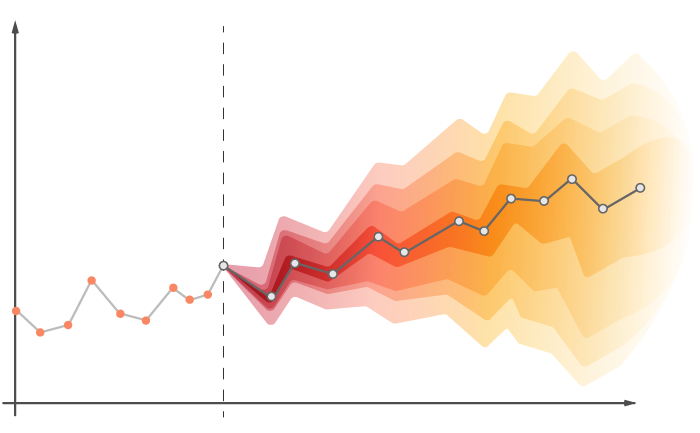
\includegraphics[scale=.5]{/Users/sebastian/IdeaProjects/thesis/paper/Figures/thesis-front.png}}
\end{figure}


\vspace{5em}

\begin{abstract}
Timeseries forecasting and anomaly detection can be done with various models. Challenges arise when the amount of timeseries to be analyzed overcomes the availability of analysts working on them. An automated system needs to be put in place to handle the ever-increasing load of today's data streams. But which models should be chosen for the dataset and task at hand? We can use one model to rule them all and deal with its downsides, or we can select the model automatically by letting yet another model decide what will perform best as shown in this work. We will explore the available models, what learning tasks commonly come to light and how a system can be designed to let inexperienced users consume these forecasting capabilities with a guided model selection while keeping the human in the loop.
\end{abstract}

\newpage
\tableofcontents
\newpage

\section{Introduction}

Many corporations process a lot of interesting data in the form of Business Timeseries. These can be customer related such as purchases, interactions through consultations, support, incident reports, usage of the service and so forth. They can also be about internal processes that cannot be attributed to a single customer, such as infrastructures providing services to multiple customers. These timeseries can provide insights on how an aspect of a company performed in the past, but they also provide the foundation to create forecasts. 

The predictions that an organization wants to make could be a single step into the future, useful for operation automation, i.e., scaling services, anomaly detection, alerting, etc. Or it is desired to create forecasts long into the future to anticipate growth, scale the business, make strategic decisions, or optimize logistics or processes.

\subsection{Types of Timeseries}

Timeseries are typically uni-variate, where we have one value per point in time. We use those values to extract the underlying patterns to be able to forecast the future horizon of that timeseries. E.g., we can collect metrics of a river's temperature every 15 minutes over the period of years. We will likely find daily and yearly seasonalities in this timeseries as the river temperature is influenced by day light and the air temperature. Thus, the temperature is colder at night and in winter.

With multi-variate timeseries we have multiple values per point in time. E.g., we can collect air temperature, level of cloudiness, air humidity, air pressure, etc. and we try to predict the river's temperature with those metrics. This is traditionally done with regression type models.

The last case is that we start with a uni-variate temperature, say the river's temperature, and we add exogenous timeseries, like the air temperature. A good model will learn the dependency between the regressor variables and the variable to be predicted. The problem now is that we need the air temperature data for the future to be available when we try to predict the river's temperature. This is not always possible. An example where it is possible is when we try to predict sales of products and we have a calendar when advertisements of the products will go online. A model could learn how the advertisement variable impacts the sales timeseries and add its effect to the forecast.

Timeseries are generally generated by collecting metrics of an underlying event stream. E.g., a timeseries on the amount of sales of a product uses each sell event as the underlying data stream. The sell events are then aggregated or binned into equally apart time slots which we will call frequency or resolution. If we choose a high frequency, e.g., 5 seconds, we will likely end up having many zeros and occasionally a one in our timeseries. In most cases this timeseries should be further aggregated into larger bins. The resolution of a timeseries needs to be chosen with its use case in mind. It is of course a good idea to record data in a very high resolution, so we have the possibility to aggregate the series further in any resolution we need later. Down sampling of timeseries is also possible, where the data points are linearly spread over smaller time slots. However, a down sampled timeseries should not be used to create forecasts because it contains inaccurate information of the distribution of metrics.


\subsection{Timeseries Forecasting Models}

Timeseries forecasting is a field that does not share many learning methods with other traditional machine learning fields like computer vision, natural language processing, speech recognition, etc. Methods like deep learning have been applied, but were not as successful, and at the same time more costly to train, than methods coming from the field. It is also hard to beat baseline methods like Na\"ive and Seasonal Na\"ive, where the model takes the last value and predicts that this is the future value. And with Seasonal Na\"ive, the last value of the same period is looked at. There are slight variations of this by taking the last, mean, median or drift, but they remain very easy to understand and are similar to what a human would do when asked to forecast a uni-variate timeseries.

One possibility to model a timeseries is with three separate components that we additively or multiplicatively combine to a prediction model. We add the trend or growth \(g(t)\) modeling nonperiodic changes, the seasonality \(s(t)\) modeling the periodic changes, the holidays and events \(h(t)\) modeling single data point effects which are potentially irregular, and the error term \(\epsilon_t\) that is assumed to be normally distributed.

\begin{equation}
    y(t)=g(t)+s(t)+h(t)+\epsilon_t
    \label{eq:fullTrendModel}
\end{equation}

This type of model is an additive linear model for example used by Linear Regression type models and Prophet \cite{prophet}. Through the nature of this component model, we can decompose timeseries as shown in figure \ref{fig:stl-decomposition}.


\begin{figure*}
\centerline{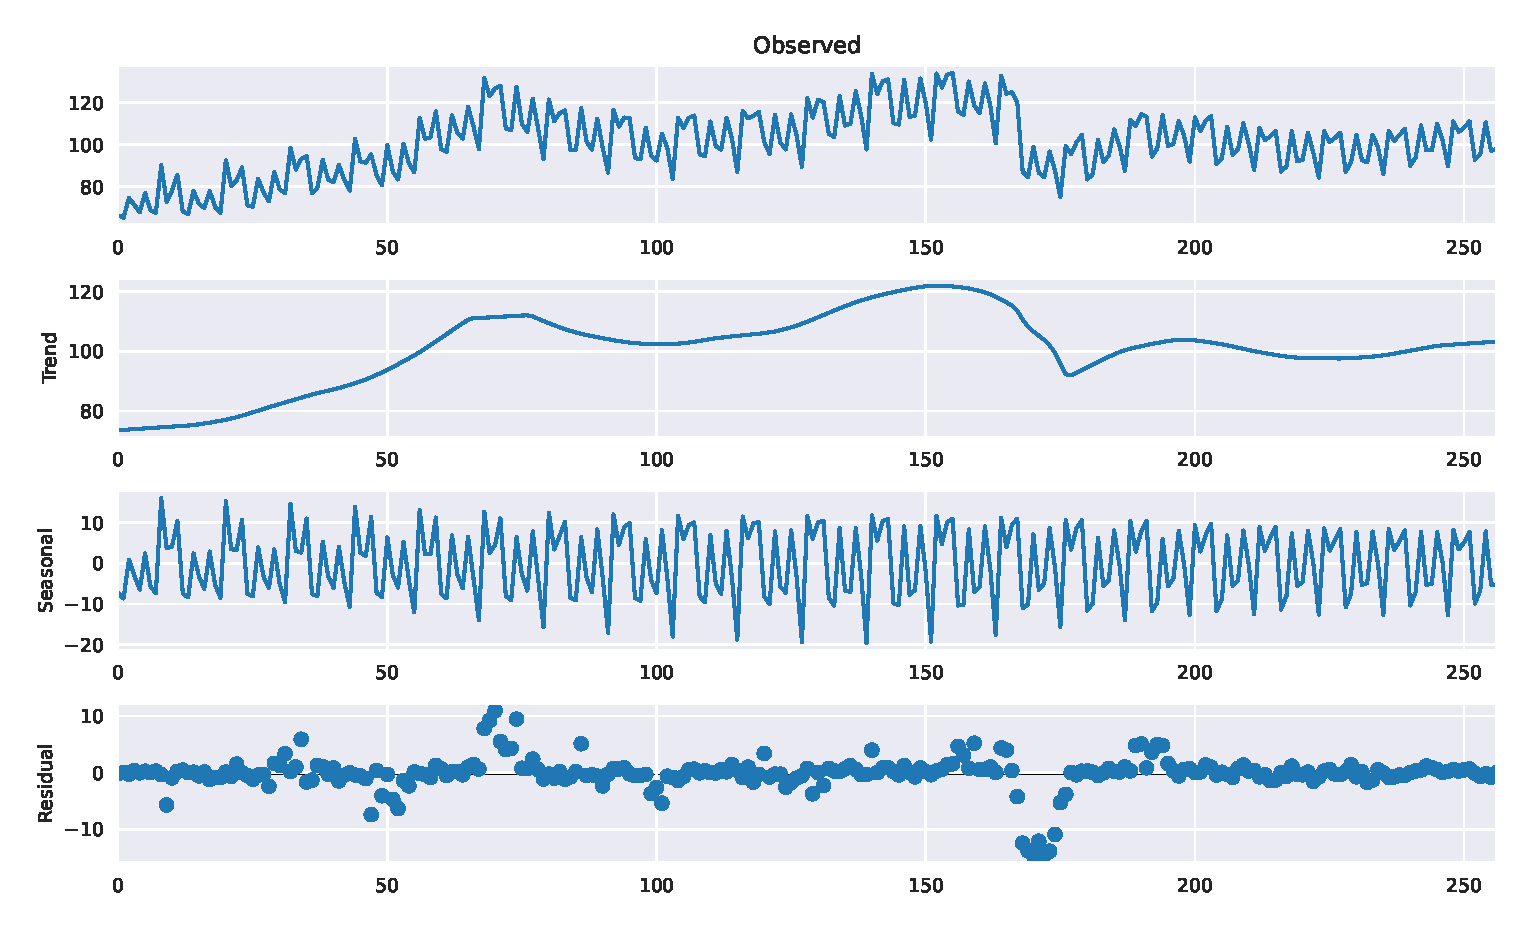
\includegraphics[scale=.6]{Figures/stl.eps}}
\caption{An example timeseries decomposed into trend, seasonal and residual components by STL \cite{STL} (Seasonal and Trend decomposition using Loess). STL works iteratively by removing a trend estimate, then smoothing the cyclic sub series to get the seasonal component. The seasonality is smoothed again, and we go back to get a more accurate trend estimate. This gets repeated several times to improve the accuracy. Such decompositions are also possible when using another model such as Prophet which uses Fourier series.}
\label{fig:stl-decomposition}
\end{figure*}

Fitting a more complex model to a timeseries does only result in a significant improvement if the chosen model makes sense for that use case and correct hyper-parameters have been specified. There are more complex models such as ARIMA \cite{ARIMA} (Auto-Regressive Integrated Moving Average) that tries to model the autocorrelations of the timeseries. Holt Winter's method \cite{HOLT} uses weighted averages of past observations, with the weights decaying exponentially as the observations get older. 
Those types of models do not include too many hyper-parameters yet specifying them correctly is not easy and only experienced analysts are capable of doing that.

Thus, it becomes time intensive and tricky to find the best model and parameters. If enough computing capacity is available and only a few timeseries shall be forecasted, we can fit a zoo of models to the timeseries and elect the best performing model. The size of a mostly complete model zoo for timeseries problems would typically be 15 - 30. But then come the hyper-parameters of each model. To truly select the best model and parameters, we need to compare all model and hyper-parameter combinations with each other in the same ranking. This grid search is expensive as the models to be fitted easily grow to thousands or tens of thousands. If fitting one model takes one second, and we are assuming we are doing this in series, we would wait hours to find the best model of a single timeseries. But we maybe have hundreds of thousands timeseries. This quickly leads to a waiting time of many years, which is not feasible. 

Another option is to select a single capable method, which performs reasonably on most timeseries and call this the model to rule them all. This approach has been taken by many companies. The model often chosen is Prophet \cite{prophet}. It can fit trends with a limiting capacity, do automatic changepoint detection, extract multiple seasonalities using Fourier series, and incorporate holiday effects into a prediction. This makes it an ideal candidate to apply to almost every timeseries forecasting problem. Using a single model has its drawbacks as well. For one, there might be timeseries in a dataset that are static, meaning they only ever contain a static value that never changes, or they follow a perfect single seasonality period. Fitting Prophet to these timeseries will likely result in a higher error term and cost more compute power than a Na\"ive method.

Timeseries forecasting is an active field of research and there are several competitions held every year to encourage people finding the best methods. The winning methods usually revolve around gradient boosted machines (GBM) with auto-regressors \cite{gbm}. These types of models are great at forecasting, but they are also inherently slow. Therefore several new optimized GBM libraries have sprouted up like LightGBM \cite{lightgbm} and XGBoost \cite{xgboost}. To win a competition, one needs to achieve the highest score, and compute cost does not matter. However, in a real-world scenario, compute cost does matter. Explainability of a model can also matter if these forecasts must be consumed by humans to make decisions upon.

Ideally, we would like to have a system that can suggest the best model automatically given the forecasting scenario, the data and the requirements in form of time, explainability and accuracy.

\subsection{Datasets}

Finding timeseries datasets initially seems trivial. When following tutorials for timeseries forecasting, the libraries usually provide an integrated or readily downloadable dataset to play around with. These toy datasets usually have been selected to highlight the strengths of a library and its default parameters, making forecasting seem easy. Real-world datasets contain a lot more error terms and hidden patterns if any. Finding a wide range of datasets with enough variation to satisfy specific needs might become a hard task.

Competition datasets usually provide a good challenge to a timeseries forecaster. Yet, those timeseries are usually made to support one forecasting task in mind, thus they do not provide a heterogeneous dataset. If one tries to fit several models to all the timeseries within such a dataset, they will probably find a wide range of winning models and a clear overall winner. However, trying to figure out which model should be selected per timeseries before trying them all out, is a hard problem, as they all have similar characteristics.


\subsection{Timeseries Prediction Tasks}

We will distinguish between different timeseries prediction tasks that will lead to different models excelling at them.

The first forecasting task is to predict the short-term future. This can be a single step into the future or several but few. E.g if we have a dataset with one data point per day, we could predict the value for the next day. Similarly, if we have a dataset with a 5 minute resolution, we could predict the data point for the following 5 minutes. In this task we tend to have less long-term dependencies and focus more on the short-term dependencies of the timeseries. The long-term trend is also not as relevant here. The error metric on the forecast will also show little differences if we use different models, as we are only predicting one point.

A harder task is to forecast the long-term future. Here we need to take trend and seasonality into account. The error metric can also easily grow as we accumulate errors over multiple data points.

Another interesting task is to find anomalies in timeseries data. One can analyze a recorded timeseries and find anomalies in the past data. There are simple methods like taking the \(n^{th}\) percentile and comparing each datapoint to check if it lies within it, otherwise mark it as an anomaly. There are also methods that use local regression (e.g., LOESS) to fit a smoothed curve and check if there are points that are outside the sensitivity bounds. We will not focus on anomaly detection in past data in this work. We produce anomalies if the incoming data is outside of forecasting bounds instead.

Anomaly Detection is also relevant in systems that produce new timeseries data points live that need to be classified as being an anomaly or not. This is typically used in operations scenarios, where a human or an automated system needs to act if there are anomalies found, as it indicates that the underlying behavior of the data has changed. This task can also be solved by methods of finding anomalies in past data, by adding the incoming data to the existing timeseries and run one of the methods over it. The other option is to forecast the timeseries a few steps into the future with a prediction bound and compare incoming data against it. If the incoming data is out of bounds, we mark the data point as anomaly. This is the anomaly detection approach what we will focus on in this work.

\section{Related Work}

In the book Forecasting: Principles and Practice \cite{fpp3} the authors that also significantly advanced the field go over the main parts of creating forecasts. It goes over the core principles that we will be using to create models for our solution. Besides the core principles, it goes over seasonal and trend decomposition using Loess (STL), auto-correlation functions (ACF), evaluation of forecast accuracy, timeseries cross-validation, regression models, exponential smoothing and ARIMA. However, they wrote this book with the intention to give the reader tools to create the best forecasts they can by manually selecting a model, choosing hyper-parameters and evaluate them using error metrics. It does not touch on the topics of AutoML or auto model selection.


\subsection{Forecasting Competitions}

% https://www.sciencedirect.com/science/article/pii/S0169207019301128
The \emph{M4 Competition} \cite{M4}, that started on January 1, 2018, and ended on May 31, 2018, follows the three previous M competitions, the purpose of which was to learn from empirical evidence both how to improve the forecasting accuracy and how such learning could be used to advance the theory and practice of forecasting. The paper analyzes the solutions used by the participants and compares it to several baseline models. Surprisingly, many teams were beaten by baseline methods, which shows that forecasting can be tricky. They also compare the computational time required to create their forecasts and incorporate baseline methods into this graph shown in figure \ref{fig:m4-time-vs-error}.

\begin{figure*}
\centerline{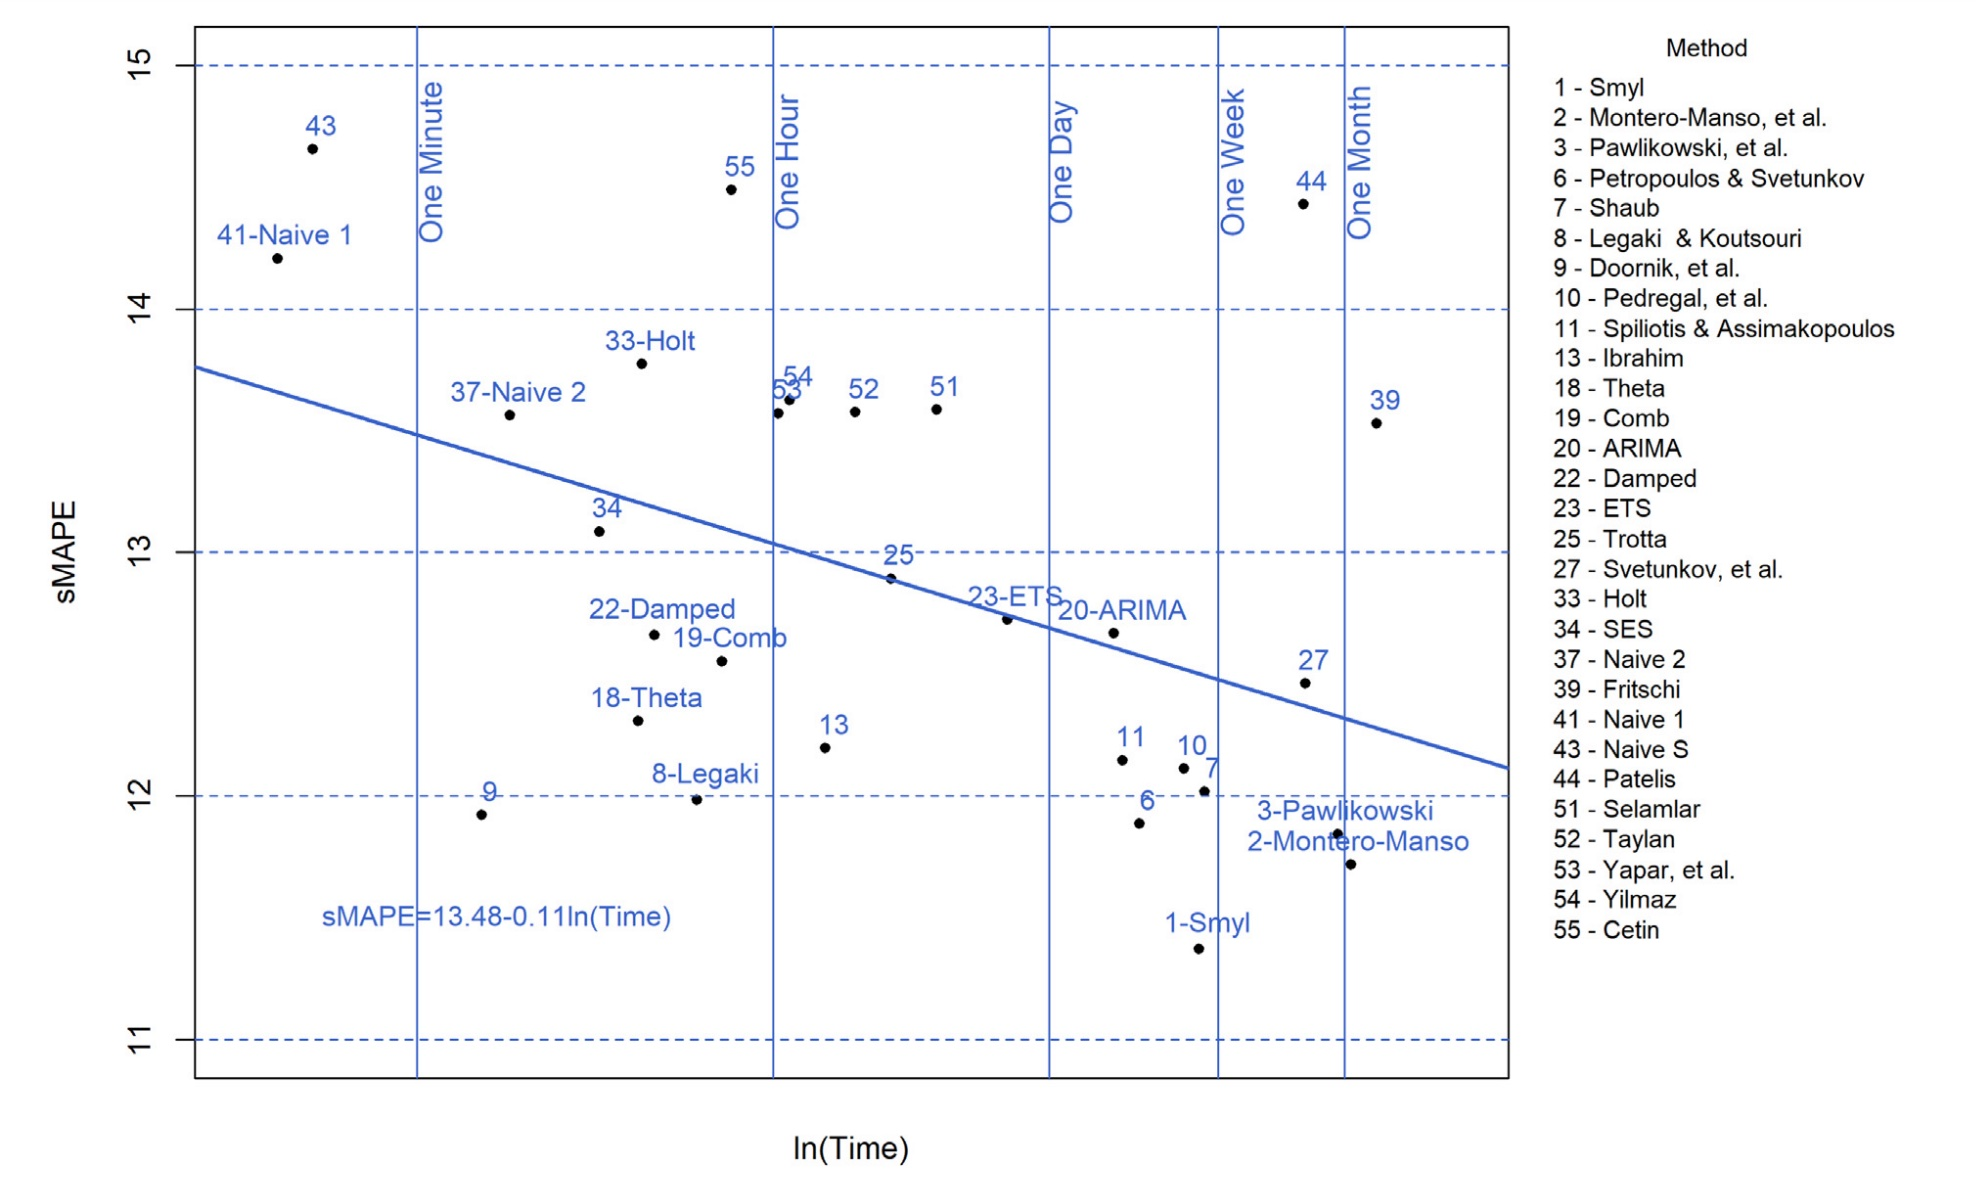
\includegraphics[scale=.25]{Figures/m4-time-vs-error.jpg}}
\caption{Evaluation of the M4 competition's winners \cite{M4}. The plot shows several baseline methods (Naive 1+2, SES, Holt, ETS, Damped, ARIMA, Comb, Theta) as well as the names of the participant groups. The dataset contained 100,000 timeseries from several sources with different resolutions from hourly to yearly that had to be forecasted. We can see that the baselines did reasonably well and outperformed most participants' methods in time.}
\label{fig:m4-time-vs-error}
\end{figure*}

The \emph{M5 competition} \cite{M5}, that started on March 3, 2020, and ended on July 1, 2020, set the competition goal to forecast Walmart sales data for around 42,000 products. The results analysis has not been published yet, but the standing can be viewed on the Kaggle leader board. The upper section of the leader board consists mostly of winners that were using Gradient Boosting machines (GBM) to create the forecasts. Until the results are published, we unfortunately do not know how long those participants let their code fit the data, except for a few ones that took multiple hours or slightly more than a day.

Google has also hosted a forecasting competition with the goal to create forecasts for Web Traffic of around 145,000 Wikipedia articles \cite{web-traffic-competition}. The winners are not required to publish how they achieved their result, however, are encouraged to do so. The first place was achieved by a seq2seq \cite{seq2seq} model. The second place went to a user of XGBoost \cite{xgboost}, a type of GBM.

These competitions lead to greater involvement of the forecasting community and ignited new research to happen. We will evaluate our results and see how they fare among the competition rankings. 

\subsection{Off the Shelf Methods}

% https://arxiv.org/pdf/2005.08067.pdf
Based on the M4 study \cite{M4}, authors of a framework embedded in the library sktime investigated how they can incorporate those results into their library. They used sktime to both replicate and extend key results from the M4 forecasting study. They can largely confirm the results and in both error metrics and time, which means we can assume that these baseline methods are hard to beat in both accuracy and compute time. The implemented framework in sktime, explained in the same paper, also allows us to profit from a coherent and re-usable API to implement a zoo of models to evaluate against our chosen datasets.

A type of model which quickly became popular in 2019 and 2020 was \emph{Prophet}. The authors of the paper \emph{Forecasting at Scale} \cite{prophet} explain the insufficiency of previous forecasting methods by taking an example time series that they recorded and tried fitting the data in an automated setting without changing the default parameters on these data. According to the authors, Prophet can work at scale because its hyper-parameters can be left at their defaults and forecasts are relatively fast and accurate. Out of their research, the authors created an R and Python library that implements the described methods and named it Prophet\footnote{\href{https://facebook.github.io/prophet/}{https://facebook.github.io/prophet/}}. In our work we compare this method to other methods and try to apply it only when it is necessary to do so. Although Prophet is quite efficient, it still requires some compute power to fit a timeseries. It also is regularly outperformed by other methods.

Based on the assumptions that baseline models perform reasonably well and that they satisfy our requirements to fit them to models at scale, without the absolute need of a human analyst, we ask the question if we can design an end-to-end system that automatically suggests the best model given the learning task at hand. Our approach needs to be at least as good as applying Prophet in terms of accuracy and better in terms of compute power required. 



\subsection{Timeseries and AutoML}

PyCaret \cite{PyCaret} is a framework to accomplish their version of AutoML. Currently the library supports classification, regression, clustering, anomaly detection and NLP learning problems. Time series forecasting is not yet in the library, but in the works as their next milestone. PyCaret's approach is to find the best model for a timeseries by fitting and evaluating a collection of models and then tune the \(n\) best models and choose the best one. This approach almost guarantees to find the best model and parameters for that task, which is great. However, fitting several dozen models onto a timeseries and then tuning them is time intensive, even if done in parallel, as PyCaret does out of the box. 

FEDOT \cite{fedot} is a library that also wants to do AutoML, but specifically for timeseries forecasting. It takes a completely different approach than PyCaret, by using evolutionary algorithms to build a pipeline. The methods used by FEDOT are limited to regression-based models. When building a model for a timeseries, the FEDOT method figures out which transformations should be used for a regression step. These input features can be Gaussian filters, smoothing, lagged variables and others. The regressor accepting these values is also selected by evolutionary algorithms. The resulting pipeline works out of the box and achieves great results. However, the fact that it's limited to regression-based models and that the evolutionary algorithm still takes several seconds to find the desired pipeline configuration. This method is interesting, but not something we can apply in our research.

Researchers at Microsoft have shown their approach on how to automatically select a model and its parameters for the narrower case of anomaly detection (AD) in their paper \emph{Automated Model Selection for Time-Series Anomaly Detection} \cite{ms-ad-model-selection}. Their method was evaluated on an internal dataset that was collected in their production. The method first extracts several features of the timeseries and creates a feature vector based on variance, auto-correlation, entropy, seasonal period and several others that are not further specified. They then trained a LightGBM model offline with that data, to be able to classify new timeseries by predicting the best AD model. In their model selection they limited themselves to only three models: SR (Spectral Residual), HBOS (Histogram-based Outlier Score) and SH-ESD (Seasonal Hybrid Extreme Studentized Deviate). This makes training the classifier much easier, since there are less classes, and thus less data needed, as traditionally the number of training data required increases with the amount of classes to predict. Their timeseries data also had human-confirmed labels if a datapoint is an anomaly or not. This makes the task supervised learning and makes evaluating the chosen model slightly easier, as they can collect binary classification metrics such as F1, Precision and Recall which will provide more clear divergence between timeseries and their best model. We will try to replicate a similar approach, but by using forecasters instead of anomaly detector models. We will also try to use more than three models.


\subsection{Timeseries Classification}

In our first approach to find the best model we will use timeseries classification to be able to predict which model to use. There are simple methods such as extracting features and fitting a classifier \cite{tsfresh} which we will try. But there are also more advanced and optimized timeseries classification models such as ROCKET \cite{ROCKET} or MrSEQL \cite{MRSEQL} that we will also evaluate. 
One branch of timeseries classification focuses on timeseries that are based on shapes. A shapelet \cite{SHAPELET} is a timeseries subsequences that is identified as being representative of class membership. Shapelets are a powerful approach for measuring phase-independent similarity between time series; they can occur at any point within a series and offer interpretable results for how matches occur. We will not use shapelets as we find that our metrics based timeseries data will not show patterns of shapes that can be compared among each other. Shapelets can for example classify timeseries that are based on the shape of plant leaves.


\subsection{Anomaly Detection}

As seen above and in several research papers, methods to do anomaly detection are plentiful. Models like HBOS \cite{HBOS}, Spectral Residuals \cite{AD-SR} developed by Microsoft and Google's methods \cite{AD-GOOGLE} likely perform very well on this task. We try to limit ourselves in this work to forecasting models and then do anomaly detection based on these forecasts. This has implications that we might not produce the best anomaly detectors out there. The advantage of forecasting based anomaly detection is that the forecast can be visualized, which can be useful in certain use cases, and then the same forecast is used to decide if a new data point is an anomaly or not. This accomplishes two tasks while fitting only one model. The visualized forecast can be used by humans to easily understand what an anomaly will be and what not, as a simple graph with confidence intervals is easy to explain.

\subsection{Anomaly Detection as a Service}

Corporations such as Google, AWS and Microsoft offer APIs or services to send timeseries data and get anomalies back. This type of API is known as \emph{AD as a service}. These corporations however do not reveal how their methods work as they are a blackbox. All companies have published blog posts or white papers, but they are not enough to be able to fully replicate their system, as they want to keep it proprietary. We will explore how those companies could have built their systems.

\section{Challenges}

We will tackle the challenges in model selection for forecasting under these requirements.

\begin{itemize}
    \item \textbf{Scale:} We want to guide model selection at scale. This means we want to support large to very large datasets with thousands of timeseries. The selected models also need to scale; thus we need to be able to figure out the model to select within a short time frame. There is no time to evaluate a series of models and select the best one, not to speak of tuning it. We could do this all in parallel on a hyper-scaler infrastructure, and make it work. But then there is a large cost to pay for the resources utilized. So, we also want to keep the cost down as far as possible when scaling up.
    \item \textbf{Accuracy that is good enough:} In our scenario, we do not want to get the highest accuracy or lowest error by all cost. The solution should be pragmatic and deliver acceptable accuracy. Making tradeoffs between accuracy and compute cost should be a user driven decision by giving preferences that are influencing the selection process.
    \item \textbf{Human in the loop:} We want a system that keeps the human in the loop but can function without a human. Models should be selected automatically, but if a human detects a problem with the forecasting that is down to the model selected, this should be overridable. We also want humans to be able to understand why a model was selected, and if other options were available at the time.
    \item \textbf{Automatic Ingestion \& Pre-Processing:} The data potentially needs to be pre-processed by transforming it from whatever the input is, to a readable timeseries format. The data might also contain outliers, and depending on the users preferences, these should be automatically removed by a simple method.
    \item \textbf{Anomaly Detection:} There might be a lot of anomalies detected in a timeseries. A user should be able to tweak the sensitivity to get less or more anomalies.
\end{itemize}

\section{Model Overview}

In this work we will evaluate a series of forecasting models against timeseries data. This section gives an overview of the models we used. The goal was to have baseline models, classical forecasting models, regression-based models, neighbor based and tree based models.


\subsection{Baseline Models}

The following models are simple, yet hard to beat baselines.

\textbf{Na\"ive:} We can further segregate this method into three modes. The \emph{last} mode, that is known as the original Na\"ive, takes the last value in the timeseries and predicts this value as the new value for however many forecasting steps we request. This mode is robust against missing data. The \emph{mean} mode takes the mean of a given window length at the end of the timeseries and predicts this value. This mode is also robust against missing data. The \emph{drift} mode takes the difference between the first and last value in the selected window and extrapolates this linearly to the forecasting horizon.

\textbf{Seasonal Na\"ive:} This method works similarly to Na\"ive but instead of going back one step, it goes back the seasonal period. E.g., with seasonal period equal to 7 it does the following: In \emph{last} mode, it predicts the value \(n-7\) as the new value. In \emph{mean} mode, it predicts the mean of the last values in that period as large as the window is. In \emph{drift} mode, it extrapolates the drift in the values of that seasonal periods linearly. This method achieves a surprisingly hard to beat baseline score in a wide range of timeseries.

\textbf{Polynomial Trend with linear regression:} This method tries to fit a polynomial curve of a given degree to the data using the least squares regression. The higher the degree parameter, the better the curve can fit the data, but the more likely it will overfit.


\subsection{Classic Models}

\textbf{ARIMA:} (Auto Regressive Integrated Moving Average) \cite{ARIMA} ARIMA models aim to describe the autocorrelations in the data. ARIMA has three main parameters: $p$ the number of lag observations included in the model, $d$ the number of times that the raw observations are differenced and $q$ the size of the moving average window. Selecting appropriate ARIMA parameters can be difficult even for experienced humans. There are methods to automate the parameter selection such as AutoARIMA \cite{fpp3}. However, as we will show later, this method is quite slow.

\textbf{Exponential Smoothing:} These methods first proposed by \cite{HOLT} model a timeseries by saying the more recent the observation the higher the associated weight. This framework generates reliable forecasts quickly and for a wide range of time series, which is a great advantage and of major importance to applications in industry. Simple Exponential Smoothing (SES) is disregarding trend and seasonality. We need to specify the initial level and $\alpha$ as hyper-parameters. However, there are methods to estimate those two parameters automatically. Trend and seasonal exponential smoothing can be achieved by splitting the equation into a level and trend or seasonality that can either be added or multiplied with each other. The full combination that also includes errors is an ETS model (Error, Trend, Seasonal). ETS can further expanded into additive, multiplicative, and damped trend, seasonality, and error which gives 9 combinations. Estimating the parameters is again difficult but automatic procedures such as AutoETS exist. Although As with AutoARIMA, these auto procedures are quite slow.

\textbf{TBATS and BATS:} \textbf{T}rigonometric seasonality, \textbf{B}ox-Cox transformation, \textbf{A}RMA errors, \textbf{T}rend and \textbf{S}easonal components \cite{TBATS}. TBATS has its roots in AutoETS but extends it further. Under the hood TBATS will consider various alternatives and fit a lot of models just like AutoETS. It additionally considers Box-Cox transformations and various amounts of harmonics used to model seasonal effects. BATS is a variant that models seasonalities with integers only. TBATS can be a model that achieves state of the art accuracy if tuned correctly.

\textbf{Prophet:} The authors of Prophet \cite{prophet} compare their methods with TBATS and state that TBATS performs badly if the parameters are left at their defaults. They search for a flexible model that has no parameters, or at least none that need to be tweaked heavily to achieve desirable results. The Prophet forecasting model is based on additive or multiplicative combination of the data's components. See equation \ref{eq:fullTrendModel}. This equation has the benefit of being computationally and cognitively simple. Also new components such as holiday effects and special events can be added. Trend is modeled as growth with \(C\) as the carrying capacity, \(k\) as the growth rate, and \(m\) as an offset parameter

\begin{equation}
    g(t)=\dfrac{C}{1+exp(-k(t-m))}
    \label{eq:simpleTrendModel}
\end{equation}

The growth rate $k$ can be replaced with a vector $a$ that contains the manually specified change points with the respective growth rate of that time interval.

The innovation that we regard as most important making Prophet a highly applicable linear model, is to allow changepoints to be in the data. The changepoints can be generated automatically, or a user can set them specifically. They model at what points the trend will change. If we introduce too many changepoints, we are not going to fit a trend correctly that lasts longer than the time frame between two change points. If we had too few, the model might result in a high error term because it does not have enough flexibility. Reducing the amount of changepoints is a regularization method.

The changepoints can be found automatically by putting initial changepoints uniformly onto the time series data. Once we have the initial change points, we put a sparse prior on these change points and compute each point's magnitude. The prior variable is a hyper-parameter that also act as regularization. Once we have the magnitudes computed we can discard change points with a low value and keep the remaining ones.

\textbf{Theta:} \cite{THETA} This method follows the concept of modifying the local curvature of the time-series through a coefficient $\theta$, that is applied directly to the second differences of the data. These become Theta-lines. Depending on the $\theta$ chosen the line approximate the long- or short-term behavior. The proposed method decomposes the original time series into two or more different Theta-lines. These are extrapolated separately, and the subsequent forecasts are combined. This method was used at the M3 competition and performed well. It was subsequently used as baseline in the M4 competition and outperformed several participants.

\subsection{Linear Regression}

We apply linear regression to create forecasts by first conditionally deseasonalizing and detrending them depending on the presence of seasonality and trend. We use seasonal decomposition with moving averages to remove the seasonal component. To remove the trend, we use a polynomial trend forecaster with various degrees. For the final regression we use several methods: Linear, Elastic Net (combined L1 and L2 priors as regularizer), Ridge (least squares with l2 regularization), Lasso (L1 prior as regularizer), LARS (Least Angle Regression), Lasso-Lars (Lasso model fit with Least Angle Regression), Baysian Ridge, Huber (robust to outliers), Passive Aggressive and Orthogonal Matching Pursuit (constraints on the number of non-zero coefficients). We have parameters to separate multiplicative and additive seasonality, degrees for the detrender, as well as specific parameters for each of the regression models.

\subsection{Neighbor-Based Regression Models}

Using neighbors to do regression is a bit exotic, but we included it to increase variety.
We use k-neighbors to do regression. The conditional deseasonalizer and detrender are prepended in the pipeline. Then the target is predicted by local interpolation of the targets associated of the nearest neighbors in the training set.

\subsection{Tree-Based Regression Models}

The simplest tree-based regression model is the decision tree. Decision trees are known to overfit the data by creating an overly complex tree that does not generalize well. There are regularization parameters such as max depth and max features. The splits are leaves can be controlled via the impurity and samples parameters. A random forest uses several decision trees on sub-samples of the timeseries and combines them by averaging to improve accuracy and avoid overfitting. Extra Trees (\textbf{Extr}emely \textbf{R}andomized Trees) unlike Random Forests do not use the most discriminative thresholds but draw them at random. Often this makes the variance lower but the bias slightly higher.

\subsection{Boosted Models}

A boosting method combines weak learners into a single strong learner in an iterative fashion. Trees are added one at a time to the ensemble and fit to correct the prediction errors made by prior models. AdaBoost performs this adaptively by changing the weights. In Gradient Boosting models are fit using a differentiable loss function and gradient descent algorithm. Those models are sometimes called Gradient Boosting Machines (GBM). Extreme Gradient Boosting (XGBoost) and LightGBM are an efficient implementation of a GBM.

\subsection{Other Models}

In our research we focus on models that could potentially compete in a realtime forecasting architecture, meaning that they should be relatively fast. There are methods that do not fulfill this requirement, as they are good at creating fixed size forecasts in big batch sizes. Multi-Layer Perceptrons (MLP) have not performed well at the M4 competition \cite{M4}, thus we did not include it. Convolutional Neural Networks (CNN) and Long Short Term Memory (LSTM), as well as other Deep Learning methods, have been applied to forecasting problems in the past, but we believe that our aforementioned methods should be able to cover our use cases. Future research can proof those methods can outperform the above models outside of niche scenarios, but as of yet it has not \cite{M4} \cite{M5}.

\subsection{Summary}

In summary, this is the list of models we evaluated: Na\"ive, sNa\"ive, Poly Trend, ARIMA, AutoARIMA, Exponential Smoothing, ETS, Theta, TBATS, BATS, Prophet, Linear Regression, Elastic Net Regression, Ridge Regression, Lasso Regression, Lars Regression, Lasso Lars Regression, Bayesian Ridge Regression, Huber Regression, Passive Aggressive Regression, Orthogonal Matching Pursuit Regression, K-Neighbors Regression, Decision Tree Regression, Random Forest Regression, Extra Trees Regression, Gradient Boosting Regression, Ada Boost Regression, XGBoost, LightGBM.

\section{AutoML for Timeseries}

AutoML is not a clearly defined term and merely means that some parts of machine learning are automated. The goal usually is that one provides raw data and the AutoML system figures out how to pre-process the data (transformations, outlier cleaning, impute data, feature extraction), fits a suitable model to it and evaluates its performance using cross-validation. The output is a deployable model that can be used to give predictions on unseen data.

\subsection{Model Selection}

One of the AutoML tasks is to select an optimal model. In timeseries forecasting we can implement such AutoML capabilities by evaluating a series of models against the timeseries data and select the best model based on some accuracy metric.

This approach is compute intensive as we have dozens of models, and each has hundreds or thousands of hyper-parameter combinations. To find the best model we have to fit all and choose the one that achieved the lowest error.

We can optimize this by fitting the least number of possible models of each type by limiting the size of the parameter grid. Once we have the best model type, we can fine tune it with a (Bayesian) optimization engine that searches the best hyper-parameters given some parameter distributions similarly to PyCaret \cite{PyCaret}.

\subsection{Temporal Test-Train Splits}

Timeseries forecasters cannot be evaluated using traditional test-train splits and cross-validation.

Timeseries data points are inherently dependent on previous points. The method traditionally used is to define a cut-off point and split the data temporally. The first part \(y_{train}\) is used to fit the model and the second part \(y_{test}\) is used to be compared to the forecast \(y_{pred}\) and compute the error term. However, this gives us only one evaluation data point. To achieve a sort of cross-validation, we can repeat this with several cut-off points. To achieve the best result, we can create forecasts at every point minus the forecast horizon \(H\) and the minimal length of meaningful timeseries data \(T_{min}\). 

Using this many cut-offs to validate a model can be costly as we must re-fit the model every time. Sean J. Taylor and Benjamin Letham proposed Simulated Historical Forecasts (SHFs) \cite{prophet} by reducing the number of cut-offs used. The generally used number of cut-off points is to create a forecast every \(H/2\) periods. This still allows the model error term to be measured and averaged which can then be compared to other models as long as a normalized metric is used.


\subsection{Evaluation of point forecast accuracy}

Because we are forecasting points and not creating class predictions, we should measure the quality of a fit by the error term \(e_{t}\) representing the difference between the observed value and its forecast. The two most used formulas are:

\begin{itemize}
    \item Mean Absolute Error: MAE = \(mean(|e_t|)\)
    \item Root Mean Squared Error: RMSE: \(\sqrt{mean(e_t^2)}\)
\end{itemize}

Both are scale-dependent, meaning they are only useful when comparing models on a single timeseries, or timeseries of exactly equal scale. Mean Absolute Percentage Error helps to remove this restriction.

\begin{equation}
    MAPE = mean(|100e_t/y_t|)
\end{equation}

MAPE is not defined when \(y_t\) is zero and has extreme values when close to zero. Symmetric MAPE (sMAPE) has been proposed by Armstrong (1978) \cite{armstrong1985crystal} to circumvent such problems. sMAPE was used at the M3 competition. However, it still suffers from zero divisions and can be negative, which does not make it actually absolute. Hyndman \& Koehler (2006) \cite{HYNDMAN2006679} proposed to use Mean Absolute Scaled Error (MASE) which was then used at the M4 competition \cite{M4}. The scale must be determined using \(y_{train}\) and taking the one-step seasonal na\"ive value for the point under evaluation. It does not specify how the seasonal period \(m\) must be determined. For non-periodical data we specify \(m=1\).

\begin{equation}
    q_j=\frac{e_j}{\frac{1}{T-m}\sum\limits_{t=m+1}^T|y_{t}-y_{t-m}|}
    \label{eq:mase_q}
\end{equation}

\begin{equation}
    MASE=mean(|q_{j}|)
    \label{eq:mase}
\end{equation}


The M5 competition used Root Mean Squared Scaled Error (RMSSE). While optimizing for MASE benefits forecasters that predict values closer to zero, optimizing for RMSSE benefits predictions close to the mean. 

\begin{equation}
    RMSSE=\sqrt{mean(q_j^2)}
    \label{eq:rmsse}
\end{equation}

For these reasons, RMSSE is the measure we will use from now on.


\subsection{Discussion}

This approach of brute force model search is not feasible if we deal if a large amount of timeseries that we need to find the best model for. As an example, let's say we have 20 model types \(m\), each having an over of 100 hyper-parameter combinations \(p_{mean}\). Then we assume an average time \(t_{mean}\) of one second to fit a model to a timeseries and produce a forecast (\(20*100*1\)). Running that would take roughly 30 minutes if not parallelized. If we only evaluate one model type at first (\(20*1\)) we improve the first part, but we might not choose the model that has the absolute lowest error in the end. After picking, we must tune the model parameters, which means that we have to try again several combinations and evaluate them against each other which maybe takes another 100 seconds if not parallelized. So, even with this optimized approach we would be billed two minutes of computing time. Therefore, we need to find the best model without running those models and seeing how they score.

We will present two approaches in the following sections \ref{sec:autoModelSelection} \emph{Auto Model Selection} and \ref{sec:guidedModelSelection} \emph{Guided Model Selection}.


\section{Auto Model Selection}
\label{sec:autoModelSelection}

Our first approach is to evaluate a lot of models against a reference dataset and record \(RMSSE\), the time it took to fit \(t_{fit}\) and the time it took to predict the forecast \(t_{predict}\) given a model and its parameters. Out of this collected data we elect the best model for each timeseries in the dataset. Given this information, we then try to setup a multi-class classification learning task. The timeseries data is \(X\) and the best model is our target variable \(y\). The hypothesis is that the timeseries themselves contain enough information to predict the best model.

In each experiment we restrict ourselves to a single but large dataset and a fixed forecast horizon.

\subsection{Datasets}

We used two datasets to run two experiments. The first dataset is the \textbf{Web Traffic Timeseries Forecasting} competition \cite{web-traffic-competition} data. The dataset consists of roughly 145,000 timeseries representing traffic to a Wikipedia article page. The resolution of the data is daily and ranges from 2015-07-01 to 2017-09-10 which is 803 data points. The task is to create a forecast from 2017-09-13 to 2017-11-13 which is a 65-day horizon. There are about 8\% of missing values in this dataset, which is not making it trivial. The page names can be grouped by language and user agent. A distribution of traffic to languages over time is shown in figure \ref{fig:wiki_lang_distribution}.


\begin{figure*}
\centerline{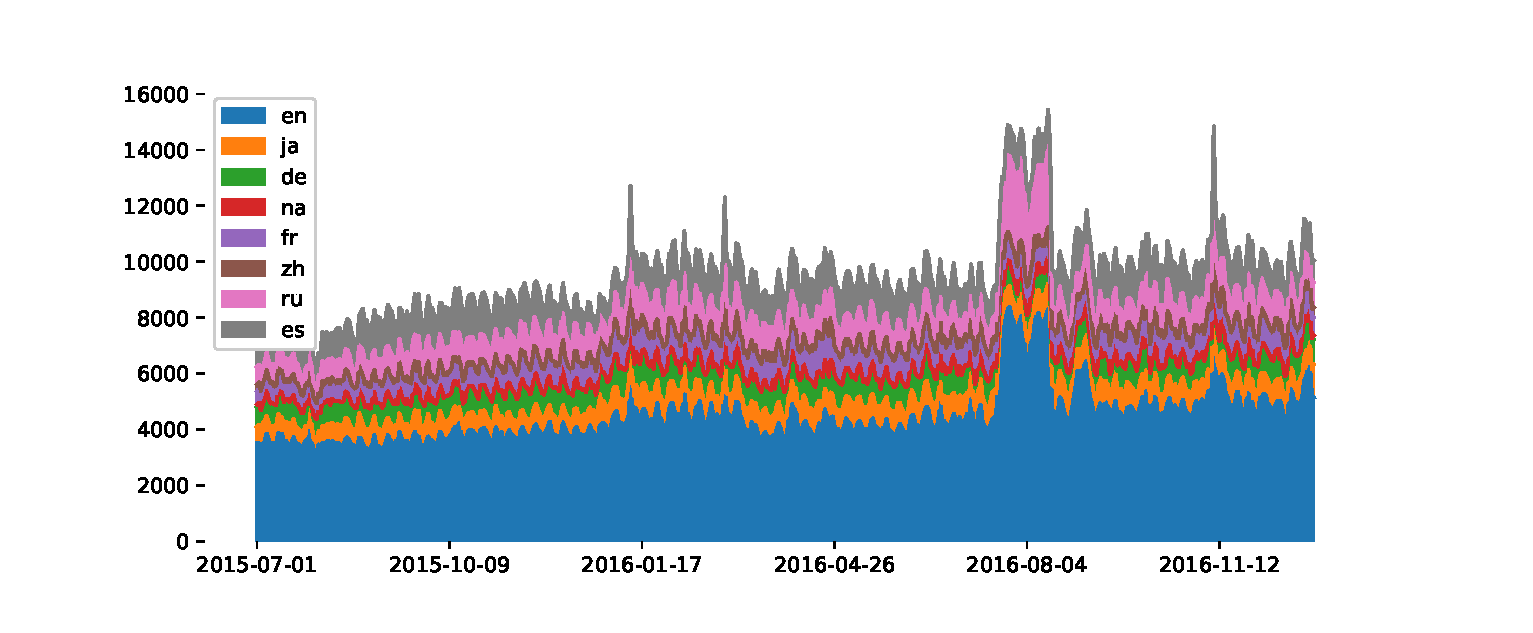
\includegraphics[scale=.6]{Figures/wiki_lang_distribution.eps}}
\caption{The Wiki Traffic dataset contains around 145,000 timeseries. This chart shows them summed and grouped by language. We find that English pages are the most common in the dataset. We can also clearly see a strong weekly seasonal pattern and a significant increase in traffic around 2016-08-04.}
\label{fig:wiki_lang_distribution}
\end{figure*}

The second dataset is the \textbf{M5 Forecasting Accuracy} competition \cite{M5} data. It consists of roughly 30,500 timeseries representing article sales. The resolution of the data is daily and ranges from 2011-01-29 to 2016-06-19 which is 1941 data points. The task is to create a 28-day forecast for each article. Many articles in this dataset went out of sale, thus we should probably predict zero for timeseries which have been sold zero times towards the end of the timeseries. A distribution of sales of product categories is shown in figure \ref{fig:m5_cat_distribution}.


\begin{figure*}
\centerline{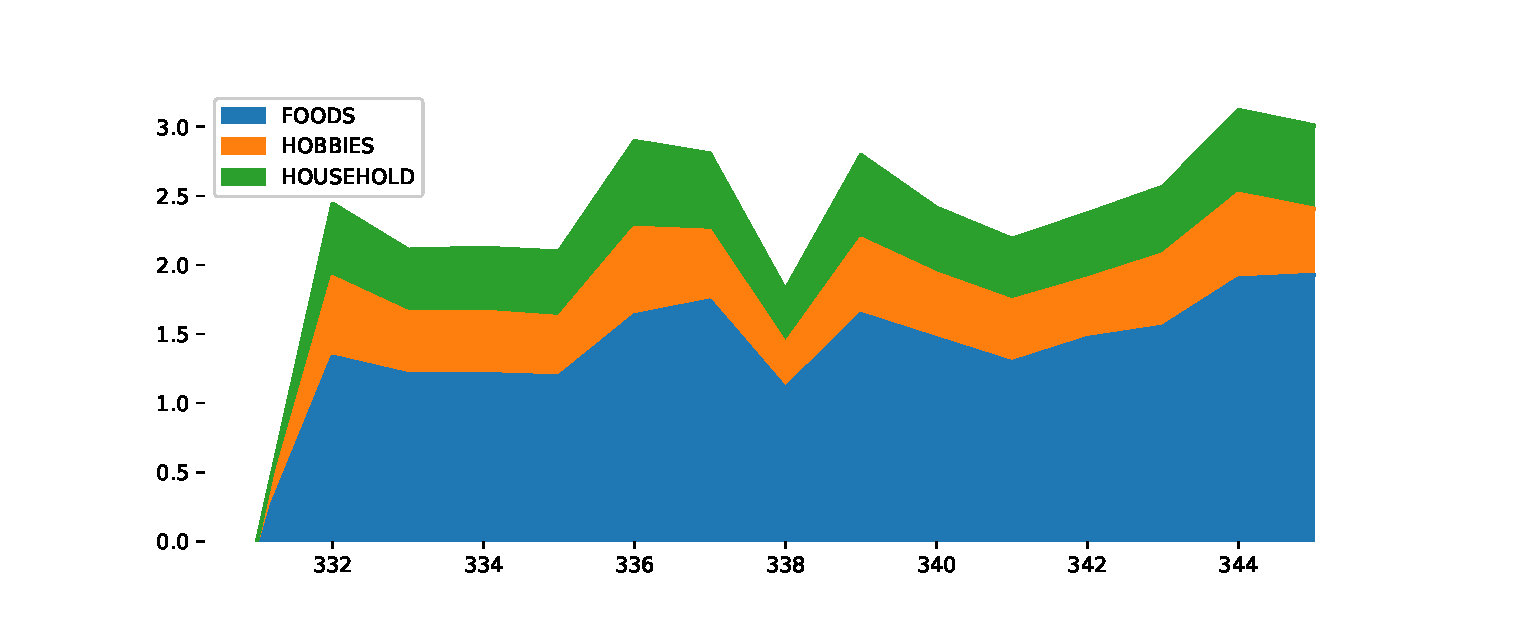
\includegraphics[scale=.6]{Figures/m5_cat_distribution.eps}}
\caption{The M5 competition dataset contains around 30,500 timeseries. This chart shows them summed and grouped by item category. We find that there is a strong weekly seasonal pattern and a general upwards trend. We also see a yearly pattern that shows food and hobby items are not being sold on a particular day. This happens to be December 25, Christmas.}
\label{fig:m5_cat_distribution}
\end{figure*}


\subsection{Evaluating Models}

We start with a large number of different models and implement each and wrap it in a common API that allows us to fit a timeseries and create a forecast. We based our implementation on sktime \cite{sktime} as they have implemented a common API for many models already. Some needed a few tweaks (Prophet) and others are regression-based pipelines that needed to be assembled. For more details which 34 models were used refer to the model overview. For each model we defined a parameter grid based on the available parameters of the model and a sensible impression that the values can make sense. We then exploded the parameter grids into all its combinations and ended up with a model of of 1451. A distribution of combinations by model type can be seen in figure \ref{fig:model_numbers}.

\begin{figure*}
\centerline{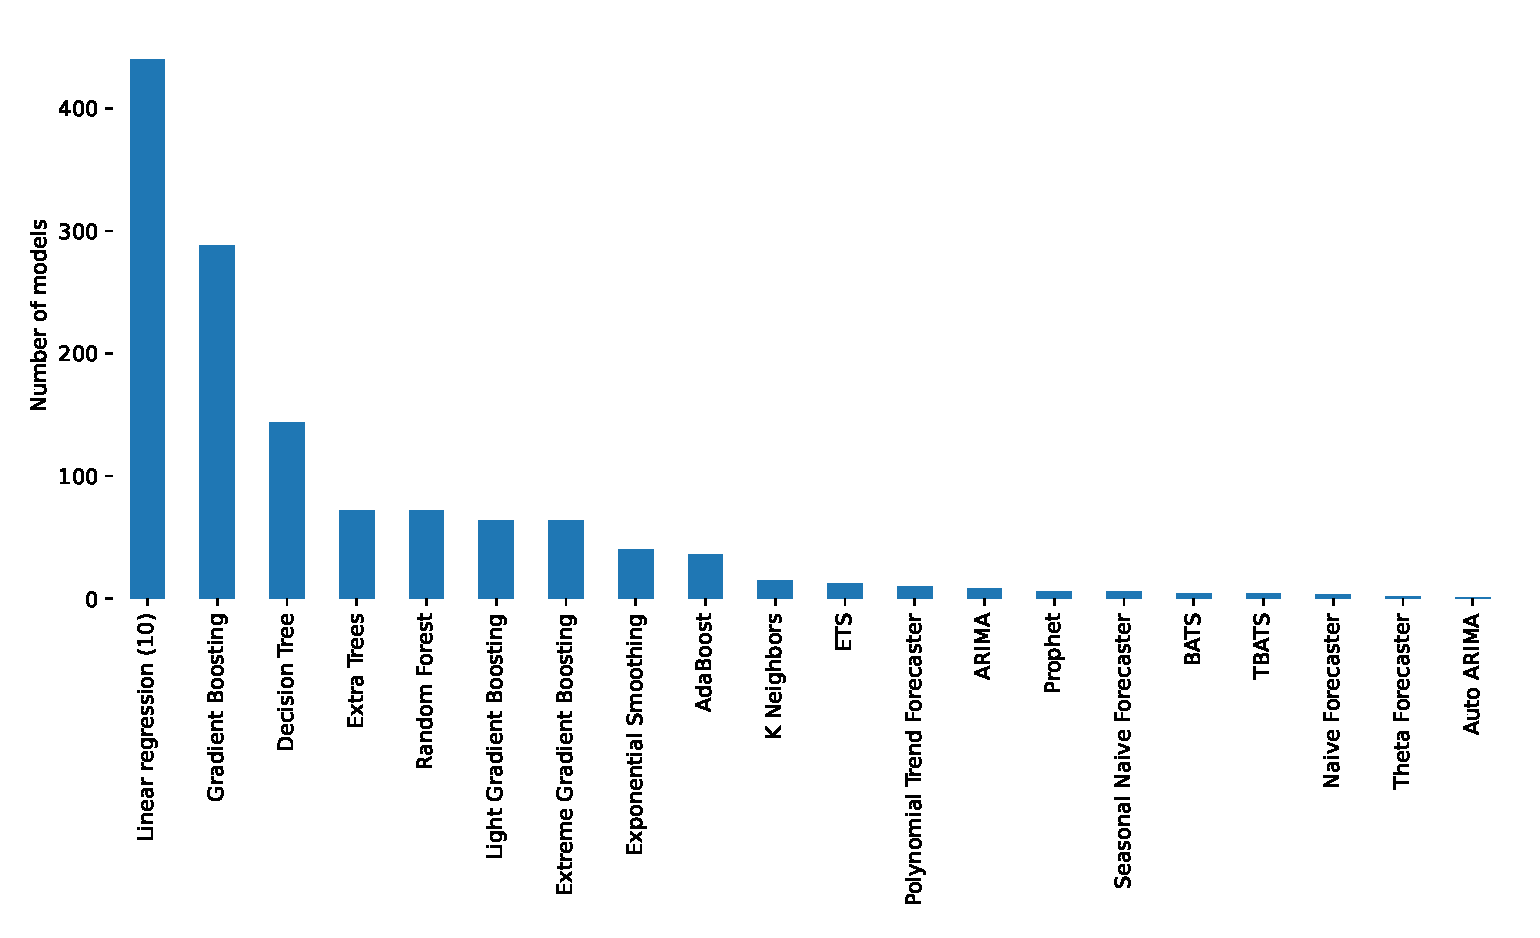
\includegraphics[scale=.6]{Figures/model_numbers.eps}}
\caption{Distribution of the hyper-parameter combinations by model. We aggregated the 10 linear regression-based models.}
\label{fig:model_numbers}
\end{figure*}


Additionally, we wanted to be able to compare models with different error metrics such as RMSSE, MAPE and SMAPE. Hence, we implemented each metric and wrapped in a common API as well. Each produced forecast error would then be computed by each metric formula.

Evaluating 1451 different models against 145,000 is not feasible. Thus, we iteratively eliminated models by selecting a small sample of timeseries and evaluating all models against it. The first ones to be removed are the models that take too long to fit. We set the threshold at 10 seconds initially. In our setup we used a Macbook Pro with a 2.6 GHz 6-Core Intel Core i7 processor. This meant the following models were removed from the list with their average fit and predict times combined: TBATS (21.s) and BATS (11.4s). For XGBoost we had to remove the n\textunderscore estimators parameter value of 300, and for LightGBM we had to remove the num\textunderscore leaves value 8 and n\textunderscore estimators value 300. We then continued pruning the models further by removing the ones with high RMSSE values and at the same time increasing the sample size as fewer models were contained in the list. 

To create labels for a classifier to learn we had to elect the best model per timeseries, for which it is important to have a large sample size of timeseries and optimally as few unique labels as possible. Unfortunately, we did not converge on a few models but had several hundreds of models that were at least once the best performing model for a single timeseries. We need to reduce the number of models. We could have aggregated by model type and ignore parameters. This however would not give good results when applying this model to a new timeseries as we either end up with an un-tuned model or we end up tuning it, which is something we wanted to avoid for time and cost reasons. We also did not want to compare models on an average error metric as they each excel at different timeseries, once they perform outstanding, and other times they produce very high error forecasts. So, we decided for each timeseries to sort the models by their RMSSE score and take the 10\textsuperscript{th} percentile best ones and increment their select score. Doing this for all timeseries gave us a score per model of how many times it was under the best performing models.

We still had models that excelled at exactly one timeseries. This leads to a problem that we cannot include models that have one attached timeseries and expect that a classifier would learn that classification. We need to reach a minimum sample size per model. Thus, we drastically reduced the number of models until we ended up with the 7 best performing models over all. The final models were AdaBoost, Decision Tree with Conditional Deseasonalize \& Detrending, Exponential Smoothing (Holt-Winters) and sNa\"ive. With their parameter combinations we had come down to 9 models. The models also nicely distributed so we had a balanced dataset. We chose the best model per timeseries to avoid having a multilabel problem besides our multiclass problem.


\subsection{Classifying Timeseries}

The next step was to build a classifier with the labels that we generated by evaluating the models. There are several methods that we tried.

\textbf{Feature Extraction:} The first method was to extract statistical features from the timeseries and use this feature vector as input to a traditional classifier. To improve our chances of finding relevant features we tried to extract as many features as possible per timeseries. The authors of tsfresh \cite{tsfresh} have implemented a vast amount of feature calculators and many possible combinations thereof. They range from mean, min, max, autocorrelation, count below x, fast fourier transform, quantiles and so forth. A complete extraction results in 4,722 features many of which are the features but with different arguments such as threshold. Some feature extractors are a bit slow however and would make this unpractical for us, since we want to classify a timeseries quickly. Thus, the reduce set of minimal feature extractors is 54. 

% TODO feature importances

We then evaluated a series of classifiers, namely decision tree, random forest and SVM \cite{SVM} to fit this data. The cross-validation precision, recall and F1 scores were unfortunately unusable. To make this Auto Model Selection approach work we would need to achieve a high precision of 80\% to 90\%. We tried to ignore the model parameters and try to classify based on model type. Yes, we said that this would not be a useful use case, but it would be interesting if there is a way to simplify the classification problem to get a relevant accuracy out of it. The result is shown in figure \ref{fig:classifier_metrics}.

\begin{figure*}
    \begin{verbatim}
                       precision    recall  f1-score   support
    
      ada_cds_dt       0.00      0.00      0.00        36
       dt_cds_dt       0.00      0.00      0.00        40
      exp_smooth       0.33      0.35      0.34        82
          snaive       0.37      0.64      0.47        92
    \end{verbatim}
    \caption{The best performing classifier was SVM. However, it only learned to separate between Exponential Smoothing and sNa\"ive. The AdaBoost and Decision Tree methods were never recognized.}
    \label{fig:classifier_metrics}
\end{figure*}

\textbf{ROCKET:} Another method to classify timeseries data is ROCKET (\textbf{R}and\textbf{O}m \textbf{C}onvolutional \textbf{KE}rnel \textbf{T}ransform) \cite{ROCKET}. ROCKET can achieve state-of-the-art classification accuracy while using a fraction of the time required by other recent scalable methods. It transforms timeseries using random convolutional kernels into features. To generate the random kernels ROCKET chooses random values for length, weights, bias, dilation and padding. The transformed features can be used to train a linear classifier. The authors recommend a ridge classifier. With ROCKET we achieved a similar result that we had with standard Feature Extraction and training a tree based classifier. We reached a precision of 32\%. We find that even by changing the method, we cannot gain better classification performance. We can say however that the ROCKET method is much faster than extracting all 4,722 features and run a tree classifier. However, if we only extract the features that are actually important, ROCKET loses out on CPU time compared to the previous method.


\textbf{Others:} We also tried other timeseries classification methods such as MrSEQL \cite{MRSEQL}, Random Interval Spectral Forest (RISE) \cite{RISE} and a k-Neighbors based time series classifier. With MrSEQL we reached the same score 32\% as with ROCKET. With Random Interval Spectral Forest and k-neighbors we both got 28\% for precision.

\subsection{Results}

We find that evaluating a large range of models and their parameters against a large timeseries dataset can be tedious. The space for optimization of this process is big. PyCaret \cite{PyCaret} is planning to ship a timeseries module in the future which could potentially be used to get faster results. However, PyCaret will only do it for one timeseries. We would still need to create an optimized evaluation execution over many timeseries.
The classification of timeseries out of one dataset has been proofed complex. The datasets we used contained all in a sense similar timeseries. This was intentionally chosen as with this approach we wanted to be able to find the best model per timeseries, not per dataset. Future research on experiment setup and tweaks to this approach might lead to better results than what we got. For us we concluded that this approach is one level too deep. Instead, we should look at the learning task parameters and the basic characteristics of the timeseries, which is a level higher, to do the model selection. This second approach is explained in the next section.

\section{Guided Model Selection}
\label{sec:guidedModelSelection}

Our second approach is to guide a human in the loop choosing the best model. We still recommend a top model that can be automatically chosen, but we have no guarantee it will perform best. Hence, we called this approach \emph{Guided}. The idea is to split forecasting tasks and its timeseries data into groups. We then evaluate several models against these grouped timeseries and again record the scores. When a user wants to create a new forecast and needs to select a model, we look at the group this forecasting task and the timeseries belong to and lookup the recommended models for this group.

\subsection{Groups}

We create groups based on forecasting task parameters and features extracted from the timeseries $T$ itself. The first variable is the user defined forecast horizon $fh$. The other variables are determined by the timeseries. We use frequency $freq$, window length $len(T)$, principal seasonal period $sp$ and if the data is strictly positive. We regard frequency as one of the base frequencies minute, hour, day, month and year. Each base frequency can have multiple resolutions, e.g., a data point every 5 minutes. The exact configurations we used are shown in table \ref{tab:groupConfigs}. Additionally, to the criteria shown there, we separate timeseries which are strictly positive or not, as this can restrict some models from working well (or their hyper-parameters).

We then create all possible combinations of these configuration parameters, which results in 580 different groups. This includes invalid configurations, e.g., the seasonal period is 365 days but the window length is only 7 days. We drop invalid combinations according to the following rules:

\begin{itemize}
    \setlength\itemsep{.1cm}
    \item Horizon is smaller than resolution
    \item Horizon is larger than the start interval of the window by a factor of 2
    \item Seasonality is larger than the start interval of the window by a factor of 4
\end{itemize}



\begin{table*}
  \fontsize{8.5pt}{8.5pt}\selectfont
  \caption{Group Configurations}
  \centering
  \begin{tabular}{p{3cm}|p{11.2cm}}
     
     Frequency & Parameters\\
     
     \hline
     \vspace{.01cm}
     Minute $m$ & 
     \vspace{-.5cm}
     \begin{itemize}
         \setlength\itemsep{0cm}
         \item Window Length: [0s, 10m), [10m, 3h), [3h, 7d), [7d, 28d)
         \item Resolution: 1m, 5m
         \item Seasonality: none, 1h, 24h
         \item Horizon: 1 step, 1h, 24h
     \end{itemize}  \\
     \hline
     
     \vspace{.01cm}
     Hour $h$ & 
     \vspace{-.5cm}
     \begin{itemize}
         \setlength\itemsep{0cm}
         \item Window Length: [0h, 24h), [24h, 7d), [7d, 28d), [28d, 5y)
         \item Resolution: 1
         \item Seasonality: none, 1d, 7d
         \item Horizon: 1 step, 12h, 24h, 7d
     \end{itemize}  \\
     \hline
     
     \vspace{.01cm}
     Day $d$ & 
     \vspace{-.5cm}
     \begin{itemize}
         \setlength\itemsep{0cm}
         \item Window Length: [0d, 56d), [56d, 180d), [180d, 480d), [480d, 4y), [4y, 100y)
         \item Resolution: 1d, 7d
         \item Seasonality: none, 7d, 365d
         \item Horizon: 1 step, 28d, 60d, 365d
     \end{itemize}  \\
     \hline
     
     \vspace{.01cm}
     Month $M$ & 
     \vspace{-.5cm}
     \begin{itemize}
         \setlength\itemsep{0cm}
         \item Window Length: [0M, 6M), [6M, 2y), [2y, 10y), [10y, 200y)
         \item Resolution: 1M
         \item Seasonality: none, 12M
         \item Horizon: 1 step, 6M, 12M, 24M, 48M
     \end{itemize}  \\
     \hline
     
     \vspace{.01cm}
     Year $y$ & 
     \vspace{-.5cm}
     \begin{itemize}
         \setlength\itemsep{0cm}
         \item Window Length: [0y, 10y), [10y, 2000y)
         \item Resolution: 1y
         \item Seasonality: none
         \item Horizon: 1 step, 2y, 5y, 10y, 20y
     \end{itemize}  \\
     \hline
  \end{tabular}
  \label{tab:groupConfigs}
\end{table*}


This gives us a list of slightly over 300 group configurations. The list of discriminative features has defined based on the insights generated by the M4 competition \cite{M4} and \cite{sktime}, that simple models can achieve almost unbeatable results in lower resolution datasets. One insight was that the baseline forecasts for the hourly data of the M4 competition was harder to beat than the daily timeseries. To also split by window length, seasonality and horizon, we hypothesize that some models that will perform worse or better depending on whether there is a lot of data available (window length), if seasonality is present and if the horizon is short or long.

\subsection{Datasets}

The next step is to find datasets which can be grouped so every group has a minimal amount of timeseries for models to be evaluated against. Luckily, we do not have to find 296 different datasets as we can ignore the forecast horizon. We can also resample low resolution timeseries to receive a higher resolution and base frequency. For the window length we can use the same series multiple times by cutting it of at the end interval of the window length. This means that the true factors making a timeseries not available for a group are seasonality, too few data points to satisfy window length and if the series is strictly positive or not.

To generate timeseries for each group we built a framework that implements a series of dataset sources, applies resampling and evaluates if the timeseries matches the group configuration requirements. Most features are easy to determine except the seasonal period.

In our scenario we used several built-in timeseries from sktime \cite{sktime} intended for forecasting (some sktime timeseries are intended for classification). These are good for daily, monthly and yearly groups. Another dataset we used is from Yahoo \cite{yahoo-dataset} and was intended to be used for anomaly detection research. It consists of about 350 timeseries with hourly resolution and 1,440 data points (60 days). We also created a wrapper for Our World In Data (OWID) COVID-19 timeseries \cite{OWID-COVID}. This data contains daily data since the beginning of the pandemic in 2020. By using the Kaggle competition datasets to forecast store sales \cite{STORE_SALES_COMPETITION} we enriched our corpus with long term daily data (3 years). For strictly positive daily data we used a dataset from a Network Traffic Analysis competition on Kaggle \cite{NETWORK_TRAFFIC_COMPETITION}. Finally, we also needed some strictly positive data in the minute frequency, which we found in climate data from the Max-Planck-Institute \cite{CLIMATE_DATASET}.

Our approach requires us to find diverse datasets that match our many groups. This can be a challenge, but we have found that it is possible for daily, monthly and yearly data. Acquiring hourly and minute resolution datasets can be a bigger challenge as those generally require more storage and open data publishers often do not expose these.

\subsection{Determining Seasonality}
% Move section somewhere else?

To split timeseries into different seasonal period groups, we need to automatically assign a seasonality as we do not have the capacity to label data ourselves. Each timeseries can contain multiple seasonalities which could be modeled using Fourier series. However, for our initial grouping we are interested in the principal seasonal period or the strongest one. 
Our approach is to compute the auto correlation function (ACF) with a maximum lag of the acceptable range for that frequency. We can then search for the highest peak with a peak finder algorithm. We require a minimal distance between peaks of 4, and minimal height difference of 0.1 and a prominence of 0.1. The prominence of a peak measures how much a peak stands out from the surrounding baseline of the signal and is defined as the vertical distance between the peak and its lowest contour line \cite{scipy}.


\begin{figure*}
\centerline{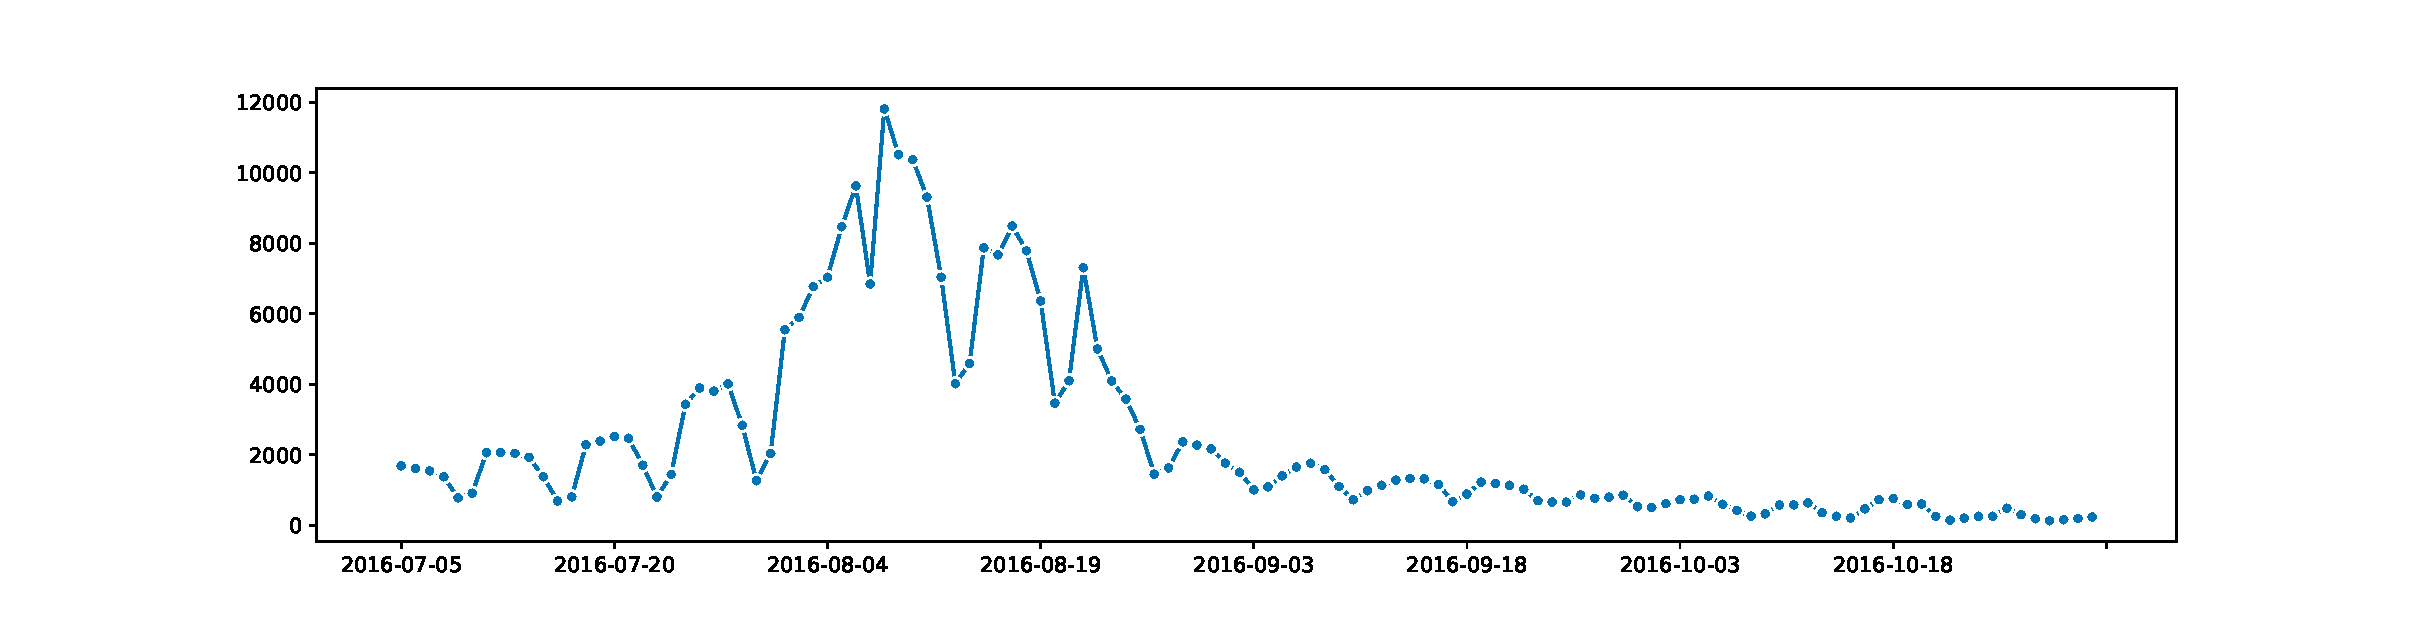
\includegraphics[scale=.4]{Figures/ts_example.eps}}
\caption{An example of a timeseries from the Web Traffic dataset that contains a weekly seasonality.}
\label{fig:ts_example}
\end{figure*}

\begin{figure*}
\centerline{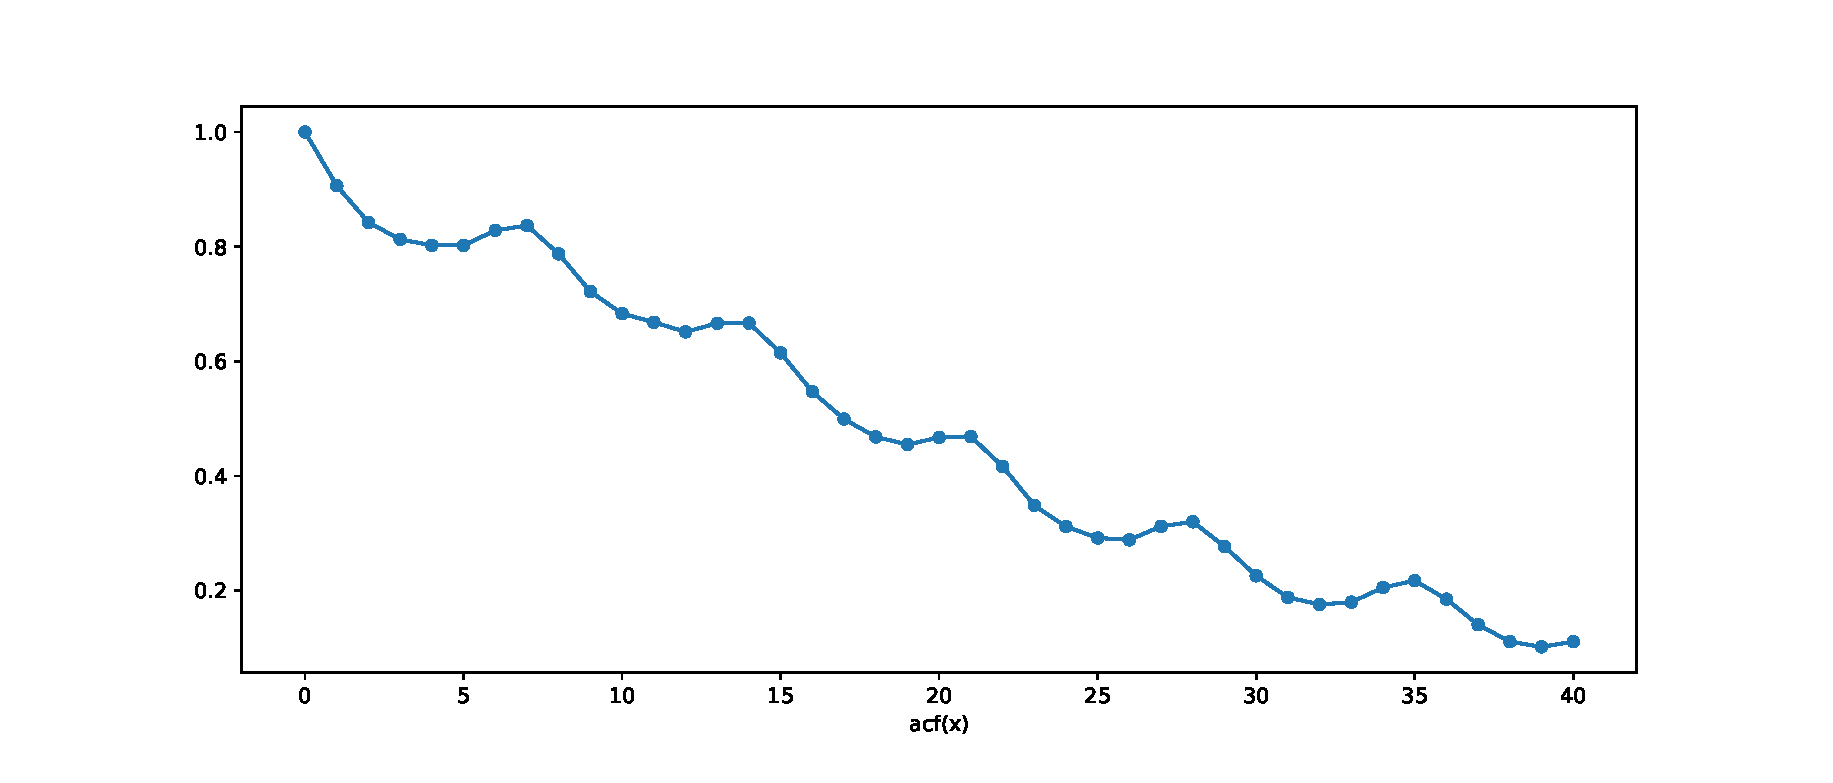
\includegraphics[scale=.5]{Figures/acf.eps}}
\caption{Auto Correlation function plot of the timeseries in figure \ref{fig:ts_example}. The initial high number at 1 is the correlation of a point with the previous point, which we are not interested in. We can see a peak at 7 and repetitions at multiples of 7. Our algorithm determined a seasonal period of 7 for this example.}
\label{fig:acf}
\end{figure*}

This gives us a list of possible principal periods. Under certain circumstances the true period was not detected as a peak but it's multiples. To mitigate this, we check if the resulted peaks have a greatest common denominator larger than 1 and include this in our list. We then filter the found peaks for acceptable periods to remove false positives. This is removing abnormal but true seasonal periods, but it has shown that doing this greatly improves the overall usefulness of using seasonality as discriminative feature.

\newpage
Our defined acceptable seasonal periods are the following. The accepted period depends on the original frequency.

\begin{itemize}
    \item Minute: 5m, 1h, 12h, 1d,
    \item Hour: 24h, 7d
    \item Day: 7d, 365d
    \item Month: 12 months
    \item Year: no periods accepted
\end{itemize}

If the ACF peak algorithm finds a period outside of this list, we reject it.

\subsection{Evaluating Models}

To evaluate models against timeseries we are using the same method from \ref{sec:autoModelSelection} \emph{Auto Model Selection}, except we are now doing it for several dataset groups. We again collect error terms, time to fit and time to predict.

\subsection{Finding Model Recommendation}

We have collected the necessary data now to recommend a model for a new timeseries. The user has several metrics available to compare the models. However, if the number of timeseries is large, we still want to automatically select a model. Just choosing the model with the best accuracy is however not the best in terms of user satisfaction. We propose that the selection is done by first mapping the metric values to metric scores $0-1$. We then create a weighting average of the model metric scores and compose a model score. The user is in control of the weights and can thus influence the chosen model. Defining the weights can be done once and then applied to all timeseries model selections.
To map the metric value to a score we use log-normal curves with specified median $m$ and 10\textsuperscript{th} percentile $p_{10}$. The following equations define our mapping function with the location $\mu$ and the shape coefficient $\sigma$.

\begin{equation}
    \mu = \ln{m}
\end{equation}
\begin{equation}
    \sigma = \frac{\ln{p_{10}}}{\sqrt{2}*0.9061938024368232}
\end{equation}
\begin{equation}
    C(x)=\frac{1}{2}(1-E_{rf}(\frac{\ln{x} - \mu}{\sqrt{2}*\sigma}))
    \label{eq:logNormal}
\end{equation}

With the score on a log-normal curve we can create scoring buckets based on percentiles. In our case we chose $[1-0.9]$ for "model recommended", $(0.9-0.5]$ for "model acceptable" and $(0.5-0]$ for "model not recommended". An example is shown in figure \ref{fig:metric-mapping}. We set the curve control points by taking the 10\textsuperscript{th} and 50\textsuperscript{th} percentiles of the metric values of that metric for that group.

\begin{figure*}
\centerline{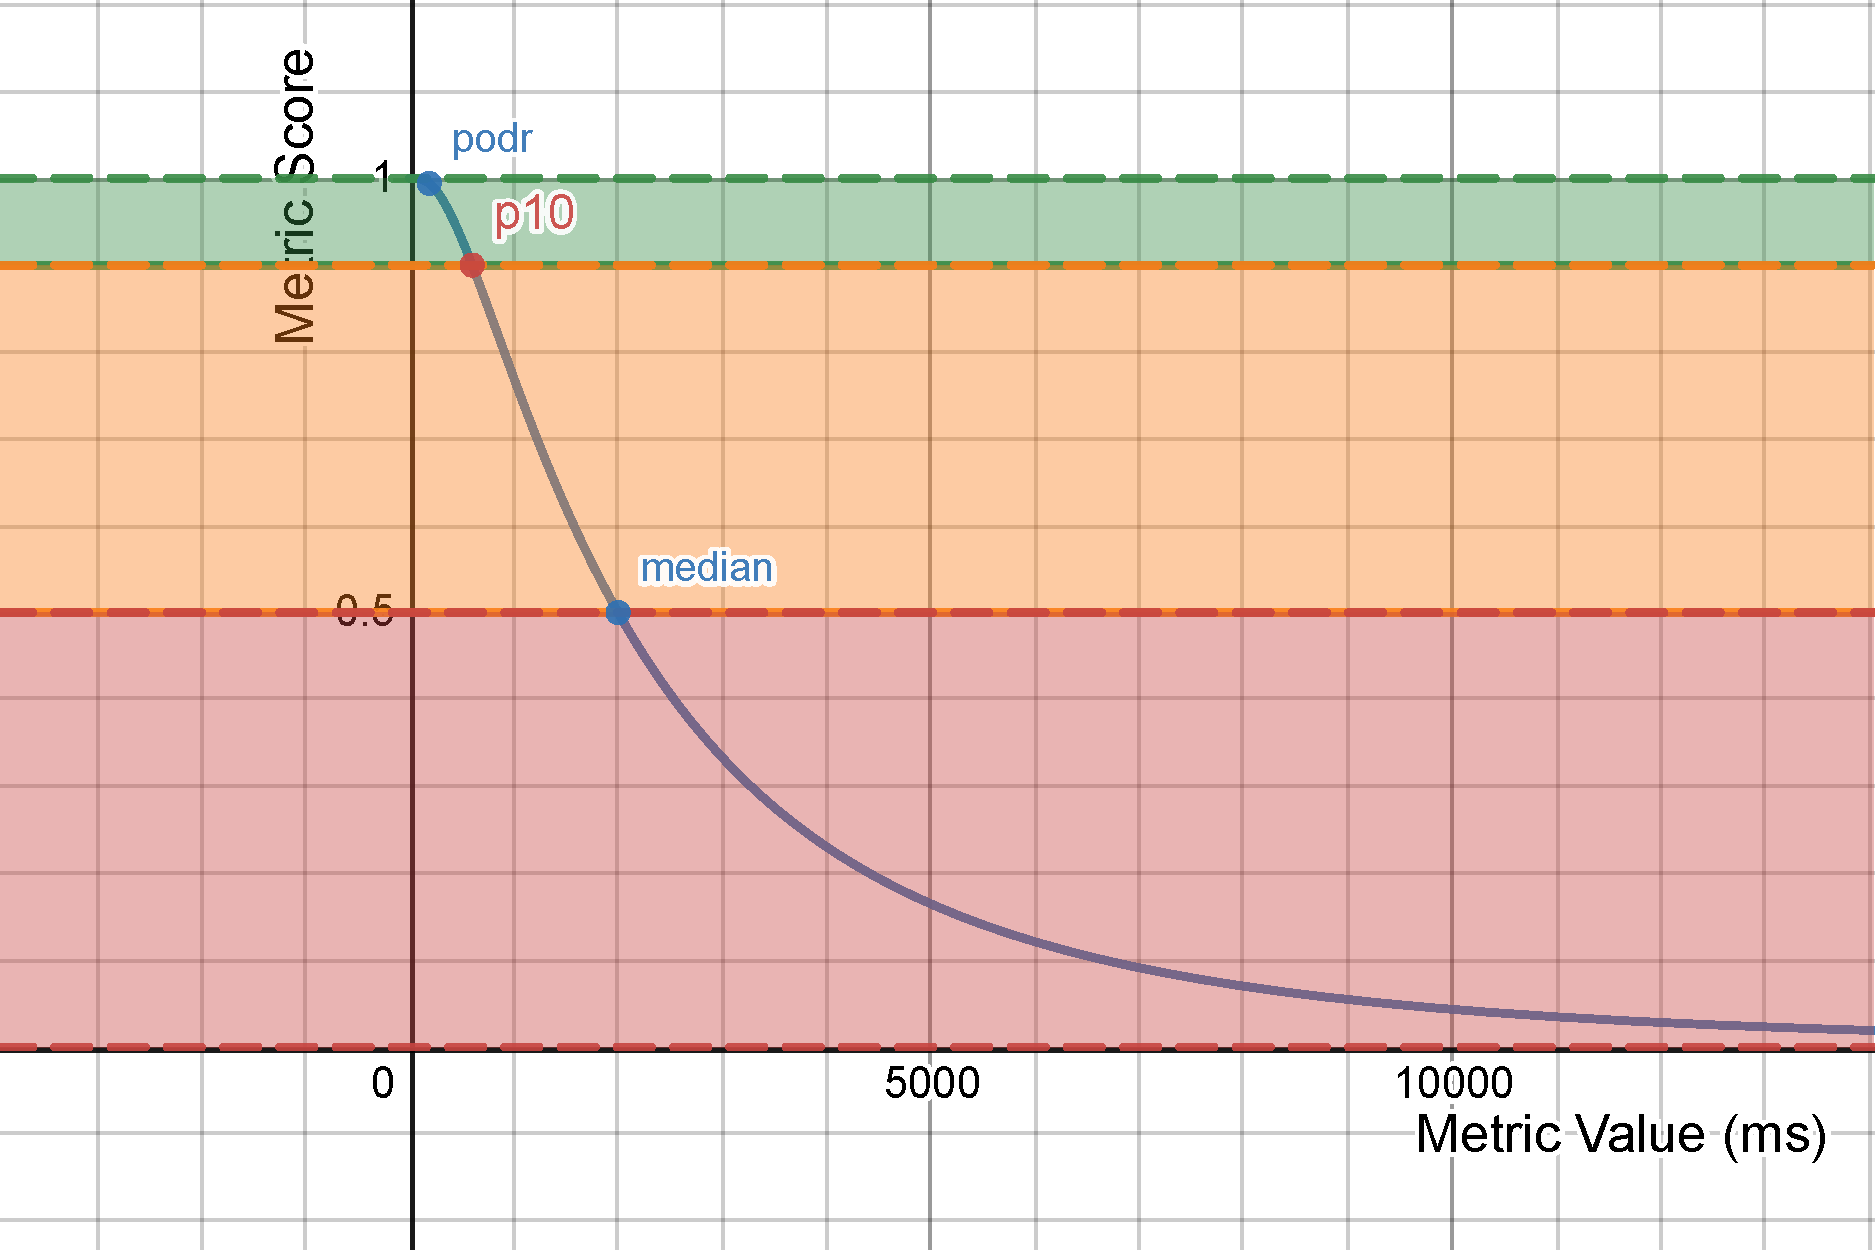
\includegraphics[scale=.33]{Figures/metric-mapping.pdf}}
\caption{The log-normal curve is mapping the metric value CPU time to a $0-1$ score. In this example we manually defined the control points $p10$ with 600ms and the median with 2000ms. The Point Of Diminishing Returns $podr$ is computed at 188ms. Meaning a model that achieves a time significantly below that is not going to get much reward for it. The upper green, middle orange and lower red section show the level of recommendation.}
\label{fig:metric-mapping}
\end{figure*}

Besides accuracy (RMSSE) and CPU time, we also assigned each model type an explainability category with scores. We used trivial ($1$), easy ($0.9$), medium ($0.8$) and hard ($0.5$) as categories. We did not find a way to determine explainability of a model other than using human perception of the model explanation itself.

Inspecting our model evaluation, we have discovered that certain model types are more consistently scoring low errors while others excel more sporadically. For example, we saw that the Poly Trend model was the best model of them all for several timeseries, but it was producing bad results for other timeseries. This is because its hyper parameter \emph{degree} is super sensitive. To change the model selection to tend towards more stable models we computed the RMSSE score for each forecast and took the standard deviation over all forecast errors. We then combine RMSSE with its standard deviation and map this to the accuracy score $0-1$ instead of just the mean.


\subsection{Results}

The resulting framework allows us to evaluate a series of models against a group of datasets and collect summaries. We can then use these summaries to decide which model we want to use by adjusting the weights for each selection variable accuracy, CPU time and explainability. With this approach we have to evaluate a range of models against a large and diverse set of datasets once, and then others can consume this in a quick, reliable and easy fashion. The decision which model to use for a new learning problem and timeseries can be computed within milliseconds, which accomplishes our initial goal. An example of a summary is shown in table \ref{tab:groupSummary}. As we will show in the evaluation section, this approach also generates final forecasts that outperform a generic model to rule them all while being fast to compute.

The quality of the summaries however depends on the diverse datasets that are used to build them. Having several hundred groups requires an assembly of datasets from different fields, different resolutions, different basic characteristics and different lengths. We were not able to find a lot of diverse timeseries data for our minute and hourly groups. But we can down sample data and shorten them to include the same source data in different groups. If we want to add more discriminative variables to split it into more groups, we will eventually fail to find data that matches these ever increasing criteria. However, we don't think that many more variables are necessary or should even be added.

In table \ref{tab:bestModelPerGroup} we show off how our proposed solution elected models solely based on accuracy per group. We find that certain models are working better in given groups than others. This proves that our used features of learning problem and timeseries create different spaces where different models work best.


\begin{table}
\fontsize{9pt}{12pt}\selectfont
\begin{tabular}{llllllr}
Freq. & $fh$ & $sp$ & Strictly pos. & Window & Winner & CPU Time \\
\hline
T    & 60min & 24h    & no  & [3h, 7d]     & Prophet        & 2,011.11ms$\pm$591.59\\
H    & 24h   & None   & yes & [7d, 28d)    & Exp. Smoothing &    34.27ms$\pm$2.19 \\
D    & 28d   & None   & no  & [4y, 100y)   & Linear Regr.   &    62.35ms$\pm$2.1\\
D    & 28d   & weekly & no  & [56d, 180d)  & sNa\"ive       &     8.56ms$\pm$1.18  \\
M    & 12m   & None   & yes & [10y, 2000y) & Linear Regr.   &    11.75ms$\pm$2.56 \\
Y    & 1y    & None   & yes & [10y, 2000y) & Prophet        &   153.52ms$\pm$31.60 \\
\ldots & \ldots & \ldots & \ldots & \ldots & \ldots
\end{tabular}
\caption{This table shows the top performing models (without their parameters) for a sample of groups. We find that data with seasonality prefers models that contain elements to handle periods. We also see that models that have a lot of data and seasonality might be forecasted more optimally by a more complex model, but it will also cost more CPU time. Some simple forecasters such as sNa\"ive will not get slower the more data they fit.}
\label{tab:bestModelPerGroup}
\end{table}


\begin{table}
\fontsize{9pt}{12pt}\selectfont
\begin{tabular}{llrrrrr}
ID & Model            & Expl.   & CPU Time        & Time Score & RMSSE           & Accuracy Score$\downarrow$ \\
\hline
32 & Linear Regr. I   & 90\%    & 62.3ms$\pm$2.1 & 43.1\%     & 0.799$\pm$0.207 & 91.3\%         \\
28 & Linear Regr. II  & 90\%    & 67.5ms$\pm$6.5 & 38.9\%     & 0.799$\pm$0.207 & 91.3\%         \\
20 & Linear Regr. III & 90\%    & 65.5ms$\pm$5.8 & 40.0\%     & 0.810$\pm$0.222 & 90.2\%         \\
24 & Linear Reg. IV   & 90\%    & 66.1ms$\pm$7.5 & 39.0\%     & 0.810$\pm$0.222 & 90.2\%         \\
10 & Exp. Smooth I    & 80\%    & 86.0ms$\pm$0.4 & 31.2\%     & 0.809$\pm$0.228 & 90.0\%         \\
49 & Theta            & 80\%    & 14.1ms$\pm$1.6 & 82.6\%     & 0.810$\pm$0.227 & 89.9\%         \\
38 & Naive I          & 100\%   & 08.6ms$\pm$1.5 & 89.9\%     & 0.722$\pm$0.317 & 89.8\%         \\
31 & Linear Regr. V   & 90\%    & 50.3ms$\pm$4.1 & 48.4\%     & 0.793$\pm$0.248 & 89.8\%         \\
27 & Linear Regr. VI  & 90\%    & 52.2ms$\pm$3.6 & 47.6\%     & 0.793$\pm$0.248 & 89.8\%         \\
37 & Naive II         & 100\%   &  8.6ms$\pm$1.4 & 90.1\%     & 0.712$\pm$0.329 & 89.7\%         \\
\ldots & \ldots & \ldots & \ldots & \ldots & \ldots & \ldots
\end{tabular}
\caption{The top models sorted by their accuracy score. The roman literals denote different parameters used for each model. This example is based on the group with daily frequency, not strictly positive, no seasonality, window length of 4y-100y, resolution 1 and a goal to forecast 28 days into the future. We can see that Linear Regression has achieved the lowest error; however it has not achieved a great time. The final ranking would be based on a weighted average score. Scores are computed using a log-normal curve.}
\label{tab:groupSummary}
\end{table}

\section{Applying it in Practice}

To show how the methods can be applied in practice, we discuss our implementation in this section.

To achieve full end-to-end AutoML for timeseries forecasting and anomaly detection that can be used by inexperienced users, we think there should be a custom built web application. A web application does not require any installation. Therefore, users do not have to setup a development environment or find a suitable cloud-based notebook solution or the like and then install a library, read the API documentation and start using it.

\newpage
The application should allow a user to specify the pipeline with as little configuration as possible. The main parts of our pipeline are the following:


\begin{itemize}
    \item \textbf{Sourcing:} In this step, the user must specify where the raw data can be retrieved from. 
    \item \textbf{Parsing:} It must be specified how the data should be read. This means telling something about the raw structure and for example which fields to read, which to ignore, and so forth.
    \item \textbf{Pre-Processing:} In the pre-processing step, the user must specify if they want to further process the raw data. This could for example be binning, time alignment, outlier cleaning, etc. but is optional.
    \item \textbf{Forecasting:} In this step, the model and its parameters are selected. This is where guided model selection comes into play and the user should be able to apply auto selection.
    \item \textbf{Anomaly Detection:} The optional step of anomaly detection uses the created forecasts and checks if new data, after the pre-processing step has run on it, matches the predictions, or lies outside the bounds. The user can accept the default sensitivity or specify a custom one.
    \item \textbf{Model Analyzer:} After the forecast was produced and new data comes in, the model analyzer can compute the error term this model had. This is a hidden step that the user does not see, except that there are metrics available per timeseries. We propose to have this step to be able to compare the performance of models over time. The analyzer can run on a schedule, intermittently or when requested by the system operators.
\end{itemize}

This pipeline should also allow to be be forked and joined between every step. Meaning, the user can define a sourcing and parsing step, and then based on the parsed data, they can define two pre-processing steps, each with different settings. This could for example be useful to create short-term forecasts with a higher resolution of e.g., hours, all the while creating long-term forecasts with a lower resolution of e.g., days. It might also be useful to join sources, if the original timeseries data is spread between different origins. Examples can be seen in figures \ref{fig:pipeline-join} and \ref{fig:pipeline-fork}.



\begin{figure*}
\centerline{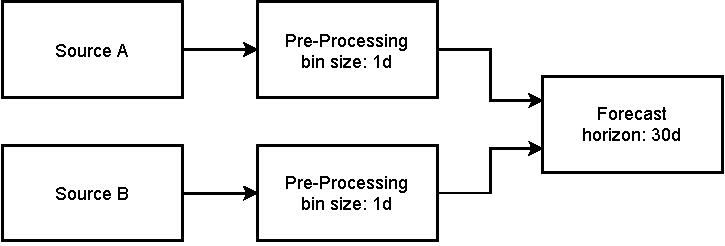
\includegraphics[scale=.7]{Figures/pipeline-join.pdf}}
\caption{Example of a pipeline that has two sources which are preprocessed independently, but then subsequently \emph{joined} to run in a single forecast step. It is the user's responsibility to ensure the sources are similar and make sense to be forecasted together.}
\label{fig:pipeline-join}
\end{figure*}


\begin{figure*}
\centerline{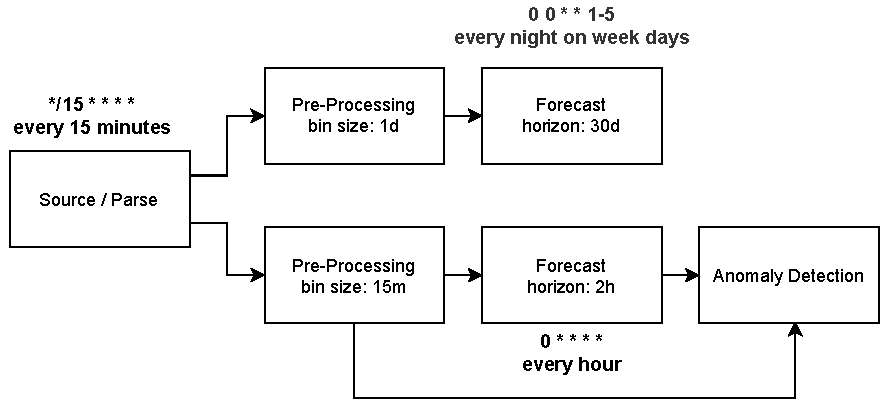
\includegraphics[scale=.7]{Figures/pipeline-fork.pdf}}
\caption{Example of a pipeline that has one source, after which the pipeline is \emph{forked}. This way users can create long-term forecasts and short-term forecasts for anomaly detection from the same source step. This means the raw data is only ingested once, which saves resources.}
\label{fig:pipeline-fork}
\end{figure*}

\subsection{Sourcing and Parsing}

The sourcing step needs to know how to retrieve raw data in the vague form of timeseries. 

This could for example be a URL that can be scraped and parsed. Or it could be a manually uploaded file. The tricky part is that the source could be in many forms. The file format could vary greatly, and even in the same file format, there are infinite possibilities to arrange the timeseries data. Thus, we must bring a lot of flexibility into the parsing step with a lot of configuration options. We also propose to split sourcing and parsing of the data. When the user is configuring a pipeline, they will need fast feedback. If they change the parsing configuration, the system should not need to download a large file again.

The aforementioned method of scraping is pull based whereas manual uploads are pushed based, although highly irregular. \emph{Pull} has the benefit of letting the system decide when to pull. This means there will never be back-pressure or processing lags in the system. However, it cannot guarantee the exact moments of data being scraped. Another drawback is that some external system needs to aggregate the data into timeseries in the first place. A push-based system, as it could be implemented with messaging techniques like Kafka, RabbitMQ and others, would benefit the producer of the data stream, as they do not need to put a metrics collection system in place. If necessary, a timeseries ingestion system such as InfluxDB, Prometheus, and so forth could be provided.

\subsection{Pre-Processing}

The pre-processing step is optional, and can transform the raw data, if desired or needed. Several pre-processing transformations make sense to apply, which cannot be figured out just by looking at the data.

Raw data can have various resolutions, and the user might be interested to collect data in higher resolutions. Thus, the pre-processing step can aggregate (also called binning) the data in bigger bins by summing or averaging the timeseries. Depending on the target bin size, it might also become relevant how those bins are aligned to time. E.g., a bin size of 15 minutes could be desired to be aligned to the full hour (0:00), the quarter hour (0:15) and so forth. We call this natural alignment which is nice for humans to consume. The analysis of the timeseries charts becomes more natural this way. The drawback when doing alignment is that the current time might not be containing all data of the most recent bin, thus this bin cannot be used yet. If we would include a partial last bin the charts will have a drop at the end, and the forecasts will most likely be heavily skewed. Consequently, if we do not include the last bin while it is of significant size yet, we cannot do near real time forecasting and anomaly detection anymore. Our recommendation would be to fork the pipeline and create two steps, one with natural alignment and one with current time alignment. The current time alignment data can be used to do near real time anomaly detection, while the naturally aligned data can be used for historical analysis.

Another pre-processing step is to fill missing data. Some models are not working well or at all when the timeseries contain missing data. Thus, by filling it in, we increase the number of models that will apply to our use case. Filling missing data in timeseries could be done with machine learning or statistical models. In fact that's how FEDOT \cite{fedot} started. As this data filling is not our main goal and only helps to increase model selection flexibility and pleases the human eye when they will later see a chart with a continuous, albeit straight line. Thus, we think back filling and forward filling are the only necessary options.

The source data could also be in absolute numbers, but the user is interested in differences per data point or vice versa. Thus, the pre-processing step should also be able to build new timeseries by building differences at various lags or to sum up differences to an absolute number (rolling sum). Some data might also be highly fluctuating, and the user would like to see smoothed data. So, moving averages of various lags should be configurable. It is important to apply these transformations before creating a forecast. One cannot assume that such a profound transformation does not affect the forecasters behavior. Our model selection will also likely suggest a different model.

Another important step besides smoothing is to explicitly remove outliers. There are several methods that can be used such as quantiles applied on sliding windows. More advanced methods, such as fitting a forecasting model are also possible, but they would be beside the point and not fast enough. We decided to use the Hampel filter \cite{HAMPEL}. It uses a sliding window. For each window of size $w$ we compute the median and the median absolute deviation (MAD). If point under observation has an $n_\sigma$-fold difference to the standard deviations, we treat it as an outlier. We can impute the point with the median to avoid missing data problems. This approach is simple, yet effective and fast. We preset the window size $w$ with 10 and $n_\sigma$ with 3. The user can adjust these parameters.

\subsection{Forecasting}

After data has been sourced, parsed and preprocessed we want to find a model for the data. The user needs to state the desired forecast horizon $fh$. The remaining features can be computed by each timeseries to figure out in which group it is. The user also needs to adjust the weights for accuracy, time/cost and explainability to create a ranking to their liking. The system will let the user choose the model of choice, if they wish to change the highest ranked model. Per timeseries, the model characteristics of accuracy, time and explainability are visible as a score $0-1$ and allow the user to base a decision on them. Scores are important for inexperienced users as they might not understand RMSSE or that different time series might lead to different CPU times required to fit the data. Once the model is chosen, the forecasting step invokes the forecaster to create a prediction for the desired horizon. The recommended model might change over time as more data is ingested. The user can enable auto selection. In this case the forecasting step first determines the group the timeseries lies in and chooses that model according to the users weights.

Some forecasters support computing prediction intervals. They are also called uncertainty bounds of the prediction. We want to store those bounds to be able to visualize them to a user. Some models do not support this feature and that's where we must use a benchmark method. We compute the standard deviation on the data that was incorporated into a forecast point. For Na\"ive this means that different values depending on the mode used (mean, last, drift). For other methods we compute the standard deviation of the window size.

Methods that support prediction intervals out of the box are Theta, ARIMA, Prophet, TBATS and BATS. If the user intends to append an anomaly detection step to this pipeline, it is recommended to use a method that properly supports intervals. Bounds produced by our benchmark method are rarely suitable to detect anomalies reliably. An example uncertainty interval is shown in figure \ref{fig:uncertainty}.


\begin{figure*}
\centerline{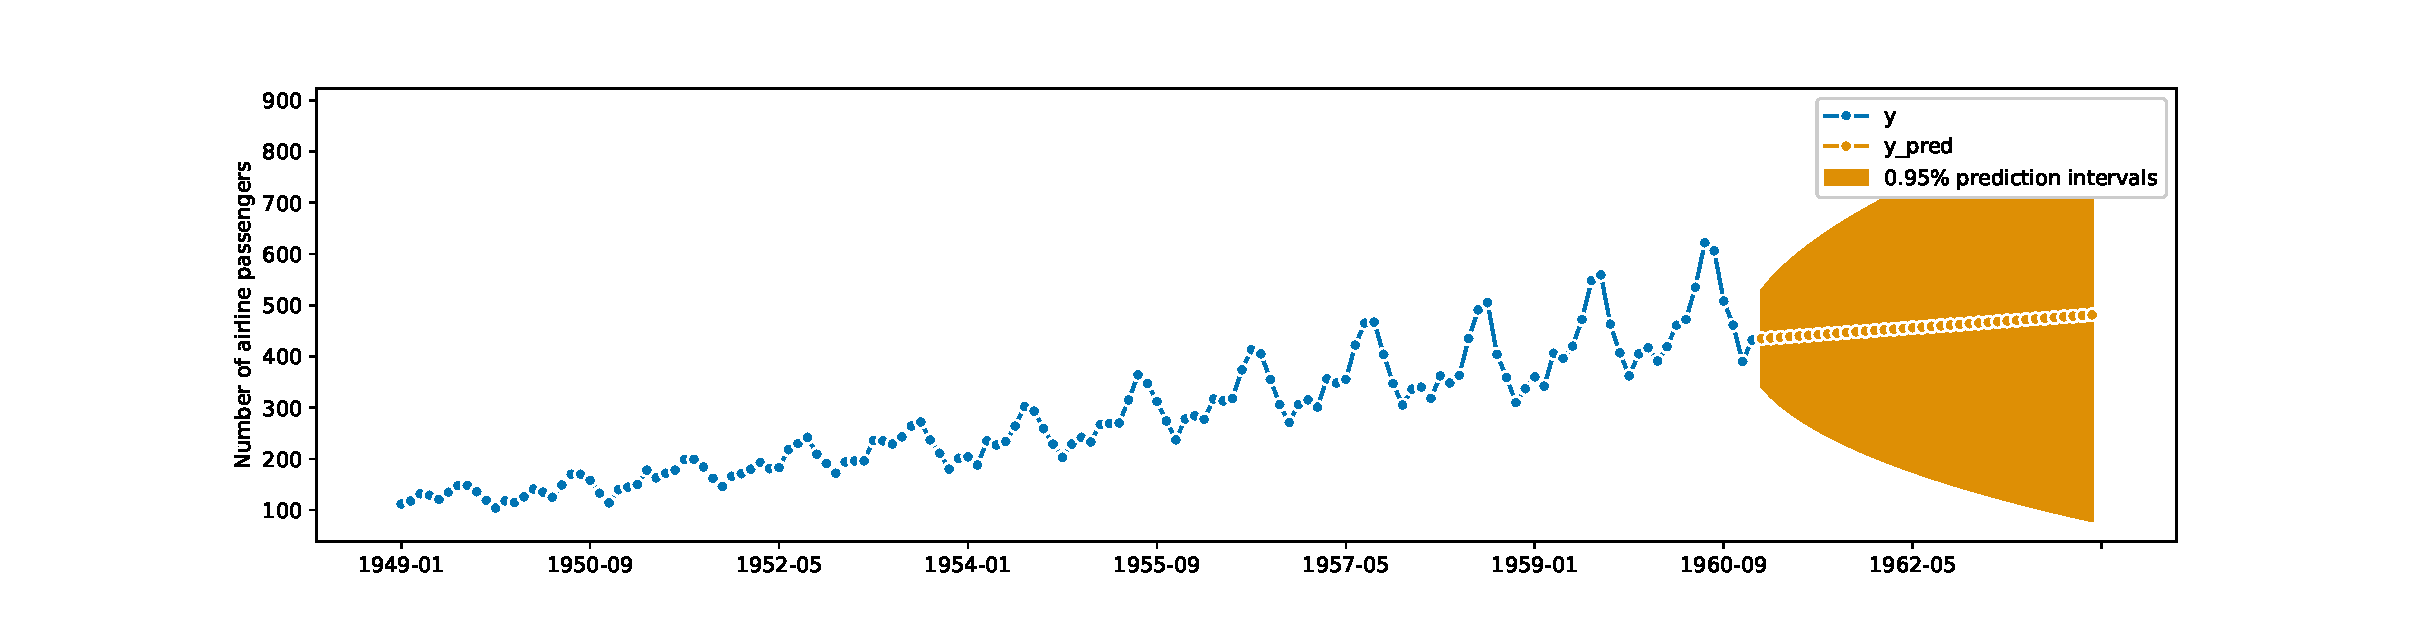
\includegraphics[scale=.5]{Figures/uncertainty.eps}}
\caption{This is an airline passenger example timeseries from sktime where we created a forecast and prediction intervals using a Theta forecaster. Uncertainty is an important factor when humans interpret a forecast. Often, forecasts can seem too correct, and humans tend to believe if they somehow find a reason to confirm the data is 100\% correct. We can also use prediction intervals to check if new data lies within the bounds or not to annotate it as an anomaly.}
\label{fig:uncertainty}
\end{figure*}

\subsection{Anomaly Detection}

The anomaly detection step uses new incoming data from the pre-processing step and compares it to the uncertainty intervals generated in the forecasting step. Users are additionally able to specify a sensitivity that can make the bounds produced by the model less strict and widen the area that is accepted to be no anomaly. A further configuration item is the duration an anomaly must occur. Traditionally anomalies are viewed as single points in a timeseries that are abnormal. But we also want to allow users to specify that something should only be regarded as an anomaly if there were a minimum of $n$ subsequent data points outside the bounds. Increasing this setting has the downside of removing the near-real-time anomaly detection aspect.

\subsection{Model Analyzer}

The model analyzer is collecting performance metrics of the forecasting method such as RMSSE by comparing training data and new data. This means that old forecasts need to be stored even though they are not used anymore, at least until the model analyzer has computed the necessary metrics.

Although we did not pursue this, by collecting these metrics, we could also run a different model on the same data without surfacing the results to the user. The model analyzer could then tell which model performed better. The system could be built to match up two competing models with every forecast until it finds the best forecaster given a timeseries in a bracket style evaluation.

\section{Scaling Architecture}

When building this system, we paid close attention to scalability. We chose AWS as a hyper-scaler platform to run our complete system. AWS provides thousands of services which are built on top of the principles of scaling and pay-what-you-use. This means if we generate intermittent load, we will only have to pay for the resources while they were in use as we do not have to provision our infrastructure for the maximum load it could ever face, and rather let it scale dynamically by demand.

Assessing the goodness of an architecture is less straightforward than evaluating forecasting accuracy. Throughout this section, we will make qualitative arguments to support our design choices by comparing it to alternative solutions and adherence to common design patterns and principles for system design and distributed computing.

\begin{figure*}
\centerline{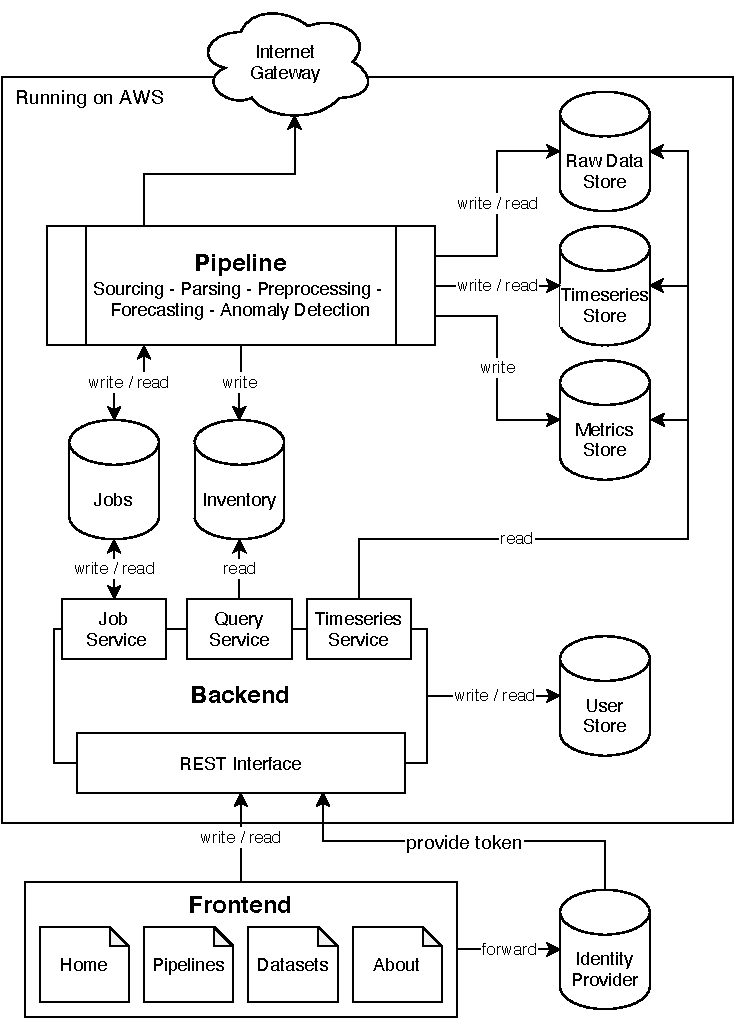
\includegraphics[scale=.7]{Figures/system-overview.pdf}}
\caption{The core components Pipeline, Backend and Frontend. All services run in an AWS datacenter.}
\label{fig:system-overview}
\end{figure*}

The diagram in figure \ref{fig:system-overview}, shows the core components pipeline, backend and frontend of the system.


\subsection{Distributed Pipelines}

Our system allows users to schedule scraping, pre-processing, forecasting and anomaly detection at any time. This means we will always have spikes in needed capacity at whatever area. Thus, we must make design choices that allow spikes to be broken down into smaller work packets that will be processed in parallel.

We propose a messaging model where events can be pushed to, and then out of it several jobs are triggered. Let's say we push ten jobs to a queue, each job then start working immediately in parallel not requiring a resource to unblock first. After a job is finished it updates the original job with its status and resource locators to the generated artifact.

Building on hyper-scaler services we can benefit from infinite amount of compute and storage resources if we implement it according to best practices. For example, a hyper-scaler such as AWS can buy more hard disks faster than a single program can write data onto such disks.

Since we want our system to have the absolute minimal costs if it's not currently in use, we also must accept some compromises. Certain open-source technologies such as Kafka cannot be provisioned on AWS without specifying a minimal broker instance type with 2 CPUs. Thus, the space of scalable messaging services is limited to services developed by AWS, if we stay with the decision to run on AWS.

Our choice for messaging and distributing the pipeline load was AWS DynamoDB\footnote{\url{https://aws.amazon.com/dynamodb/} (30-10-2021)} and AWS Lambda\footnote{\url{https://aws.amazon.com/lambda/} (30-10-2021)}. AWS DynamoDB is a proprietary document store like MongoDB. One can store documents of any shape in a table as long as they contain a partitioning key and an optional sort key. We can then enable streaming of a table to trigger events automatically by the system. In our case we trigger executions of AWS Lambda serverless functions. Lambda functions are pieces of code that do not have a known host instance. Once invoked, the platform allocates the required resources on a node and pulls the code package and executes it. After the function is done, the Lambda services keeps its allocated resources and placed code warm for a bit longer to profit from a startup boost should there be another invocation soon after. 
DynamoDB is priced with \$1.25 per million write requests, \$0.25 per million read requests and \$0.25 per GB-month. We do not need to keep logs of jobs forever and we should evict them after a while. In DynamoDB one can set a Time-To-Live (TTL) per document in a table.

In our proposed architecture, multiple actors can publish a job in a job queue of a certain type (Sourcing, Parsing, Preprocessing, Forecasting, Anomaly Detection, Model Analyzer). Each job has its own DynamoDB table, and thus we can trigger different functions based on the table. Spikes in new job creation do not matter as AWS Lambda spawns as many functions as necessary. The function invocation event also contains the content of the document itself, in this case the job description, meaning we do not need to read any job configuration upon invocation. 
The default pipeline is shown in figure \ref{fig:pipeline-diagram}.

There are three types of job creations. 

\textbf{Manual} invocation happens if the backend needs to have a job processed immediately when a user is currently configuring a pipeline and wants fast feedback. We considered storing manual jobs in a separate queue, but in the end, this is not necessary because jobs are processed immediately in any case. It would only make the architecture unnecessarily more complex. We added a preview flag to these jobs. If the flag is set, the step will only compute a partial \emph{preview} result that can be shown to the user as fast feedback to their configuration. We set the number of timeseries to be processed in a preview to a maximum of 10 first rows.

\textbf{Scheduled} invocation happens if a job has been configured to run on an interval. In our case we use the Cron \cite{cron} notation to specify a schedule. To support scheduled jobs, we need an extra piece in our architecture. We do not want to trigger the target functions directly by adding a scheduled trigger, because then they would need to get the job information in this case, and we lose our decoupling through the job queue partially. Thus, we have another function which is triggered by the configured schedules in the system. It then computes which jobs must be executed and writes them into the respective queues. Sourcing, Forecasting and Anomaly Detection steps can be triggered by a schedule. Additionally, every step that follows a pipeline join must also be triggered by a schedule.

\newpage
\textbf{Downstream} invocations happen when a step in the pipeline finishes, such as sourcing, and another step down the stream now has to process the data, e.g., the parsing step. To solve this and keep our decoupling, we added yet another function which listens to a stream of job updates of steps that can have downstream steps. We call this the scheduler function. It can then put the follow up jobs into the respective queue. There are multiple downstream steps if the pipeline is forked.

\begin{figure*}
\centerline{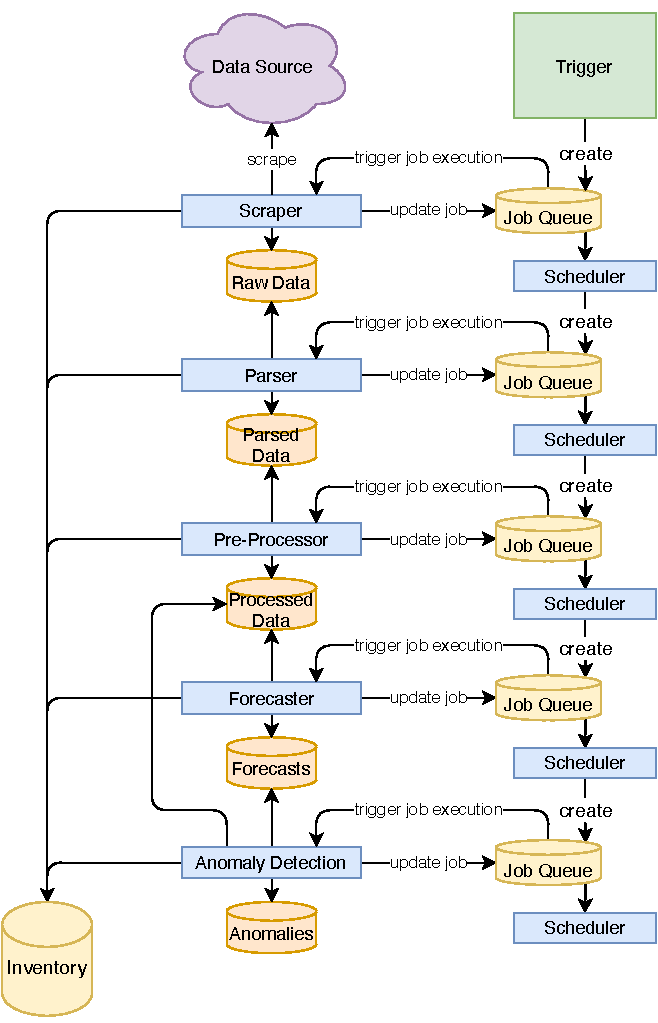
\includegraphics[scale=.7]{Figures/pipeline-diagram.pdf}}
\caption{The default pipeline is shown in this diagram. Each step can only be triggered by adding an item to the job queue. A step also never directly triggers any other steps. Everything is decoupled using message streaming. The blue boxes are implemented as AWS Lambda functions. The Orange stores are AWS S3 buckets. The yellow stores are AWS DynamoDB tables.}
\label{fig:pipeline-diagram}
\end{figure*}

We store artifacts in AWS Simple Storage Service (S3)\footnote{\url{https://aws.amazon.com/s3/} (30-10-2021)}. These artifacts are raw data scraped from a URL, processed timeseries in the form of CSV files, forecasts and anomalies also in the form of CSV files and metrics of the model's performance in the form of JSON files. The forecast CSV file contains the timeseries data used to predict it but is labeled with a flag in an extra column. The same applies for detected anomalies. The anomaly detection step will create a new CSV file with original data, forecasted data and anomalies. Each step may also update the inventory store which keeps track which dataset and which timeseries exists and where to find this data on S3. When the backend wants to display a timeseries with original data, forecast and anomalies, it only must fetch the last CSV file from S3 in a single get operation.

We are not using a timeseries database such as AWS Timestream, InfluxDB or the like. We argue that it is not necessary to have a timeseries database in our case. A timeseries database allows to make queries of timeseries data that includes filters, transformations and aggregations. We do not need to aggregate multiple timeseries, nor do we need to transform them, since our pipeline's job is to apply necessary transformations already. We need to lookup them up, but we propose to use an Inventory approach where we store the keys and labels in a DynamoDB table that can be searched. Most timeseries databases are also focused on ingestion and recent data, where they compact older data to save storage space. We do not want a database to compact old timestamps, as they might have been uploaded by a user just recently and are in high use.

\subsection{Pipeline Latency}

The data sourced is potentially many megabytes large containing thousands of timeseries. Computing a forecast on all of them at once in a single AWS Lambda function is not a good option to keep the pipeline latency low. Thus, we propose to use smaller batch sizes. Steps other than forecasting do not need batch processing as they are generally all fast or can inherently not be split. Before creating the forecasting job, we split the dataset into timeseries and group them according to their selected model which is defined in the pipeline configuration. We then create batch sizes according to the expected time per forecaster to fit and predict such that the total execution of the function remains less than 5 minutes. We have the expected durations recorded in our summaries from the model evaluation, thus we make use of them. Each function then receives a batch range that it uses to read only those timeseries from the dataset in S3. This allows us to keep the latency of the produced forecasts relatively low. Because we have now multiple functions working on the same step of the pipeline, we now have not only a pending and complete job, but each function will update the job and marking the batch as complete. The function that updates the job as the last function notices that all other batches are also complete and marks the job as fully complete. For this case it is important to use strongly consistent database reads in contrast of eventually consistent reads (which is the default for DynamoDB).

However, we run into a problem if we must create forecasts for a dataset such as the one from the Web Traffic competition with 145,000 timeseries in it. Assuming the user selects a model for all timeseries that is comparatively very slow such as 2 seconds. We then estimate a batch size of 150 to allow the function to finish within 5 minutes. This means we will spawn $145,000 / 150 = 966$ functions. The limit of AWS Lambda functions that can be running at the same time is 1,000 by default. To mitigate this, we increase the batch size for such datasets, so forecasts are ready within 15 minutes. AWS allows the increase of the concurrently running Lambda functions if necessary.

\subsection{Backend}

Our web application needs to have a backend. We propose to use the Backend-for-Frontend (BFF) design pattern. In this pattern, a frontend only ever has one backend it communicates with and vice very, the backend only has one frontend. The benefit of using this pattern is that all the endpoints can be built tailor made for the frontend and there is no need to build a generic API that does not work well for the frontend.

Our backend exposes a REST API that uses OAuth 2.0 \cite{oauth2} to protect certain endpoints which need authentication and authorization. Our technology of choice is Java and Spring Boot, however this does not really matter as other languages and frameworks are out there that do the job just as well. It is important however that these applications can be containerized and are cloud native. We are using a stateless API which means we can dynamically scale horizontally if load for the backend increases. We run our backend with AWS App Runner\footnote{\url{https://aws.amazon.com/apprunner/} (30-10-2021)}. This service handles complexities like resource pool allocation, load balancing, auto scaling and automatic deployments with a rolling strategy which does not incur any downtime when a new version is deployed. There is no need to specify or maintain a cluster. It is close to using Cloud Foundry\footnote{\url{https://www.cloudfoundry.org/} (30-10-2021)}. If we would use a popular alternative Kubernetes\footnote{\url{https://kubernetes.io/} (30-10-2021)} we would need to handle this by configuring and testing every aspect. In our scenario we do not need the flexibility that Kubernetes offers; AWS App Runner is good enough.

To expose our REST API to the frontend we configured AWS CloudFront\footnote{\url{https://aws.amazon.com/cloudfront/} (30-10-2021)} to be our entrypoint for incoming requests. The CloudFront distribution then routes requests which begin with $/api/$ to the backend URL. The backend URL points in fact to a load balancer which distributes the load between the backends and measures the traffic to do auto scaling.

\subsection{Frontend}

Above we mentioned CloudFront. If the path does not begin with $/api/$, we proxy to a S3 bucket which contains the built sources of our web application in HTML, JS and CSS files. We build these files by using Angular\footnote{\url{https://angular.io/} (30-10-2021)} as a frontend framework to implement a Single Page Application (SPA). This application allows users to sign up, configure a pipeline and inspect the resulting forecasts. The fact that this is a highly interactive website and that it communicates with a REST API lets us argue that a SPA is a good fit.

Users need to authenticate to create pipelines. We did not plan for one-off visits where a user creates one forecast and then leaves the sit and never wants to tweak their pipeline. Our system allows signing up through Google OAuth 2.0 \footnote{\url{https://developers.google.com/identity/sign-in/web/sign-in} (30-10-2021)}. The benefit is that users do not need to create an account by entering username and password. The drawback is that users need to have a Google Account. We want to extend this sign-up process to support more providers such as GitHub and provide a fallback for email and password if the user does not want to sign up using any of these identity providers.

Users can make their datasets public. This means that unauthenticated users can access these timeseries and their forecasts. This can be useful if the data is open-source and one wants to consume forecasts about certain data.

\section{User Interaction}

An important part of making forecasting available for inexperienced users is the way the user interface is built and how easy it is for newcomers to interact with it and achieve the desired results. The solution should be easy to grasp but let users explore further if they are interested in becoming a power user. In this section we go through the main parts of our frontend.

\subsection{Pipeline Configuration}

The first step a user must do to get started is to create a pipeline. This is also where we expect most users to give up already if they do not achieve any results within minutes.

As discussed before, our pipeline is flexible, has many steps and can be forked and joined. This is complex to understand for a user that just wants to create a forecast. Thus, such powerful but optional tools should be placed outside of the common flow that guides the user through the UI.
When configuring a pipeline step, it is imminently important to give fast feedback to users. Fast feedback gives a sense of trust. When specifying a URL to scrape a file, the result is a report that the file was successfully downloaded, how long it took, with what bit rate and how large the final file is. For parsing, we show a preview of the resulting timeseries by listing the top ten extracted timeseries including charts. For pre-processing we show a preview of the transformed timeseries before and after the transformation.

The forecasting step allows the user to choose a model. However, we expect that most users are not interested to change the forecasting model. They will probably also leave the weights to get the average model score as they are preset. Thus, we fill everything with defaults and if the user does not want to change anything, they can just continue. A screenshot is shown in figure \ref{fig:pipeline-config-screenshot}.


\begin{figure*}
\centerline{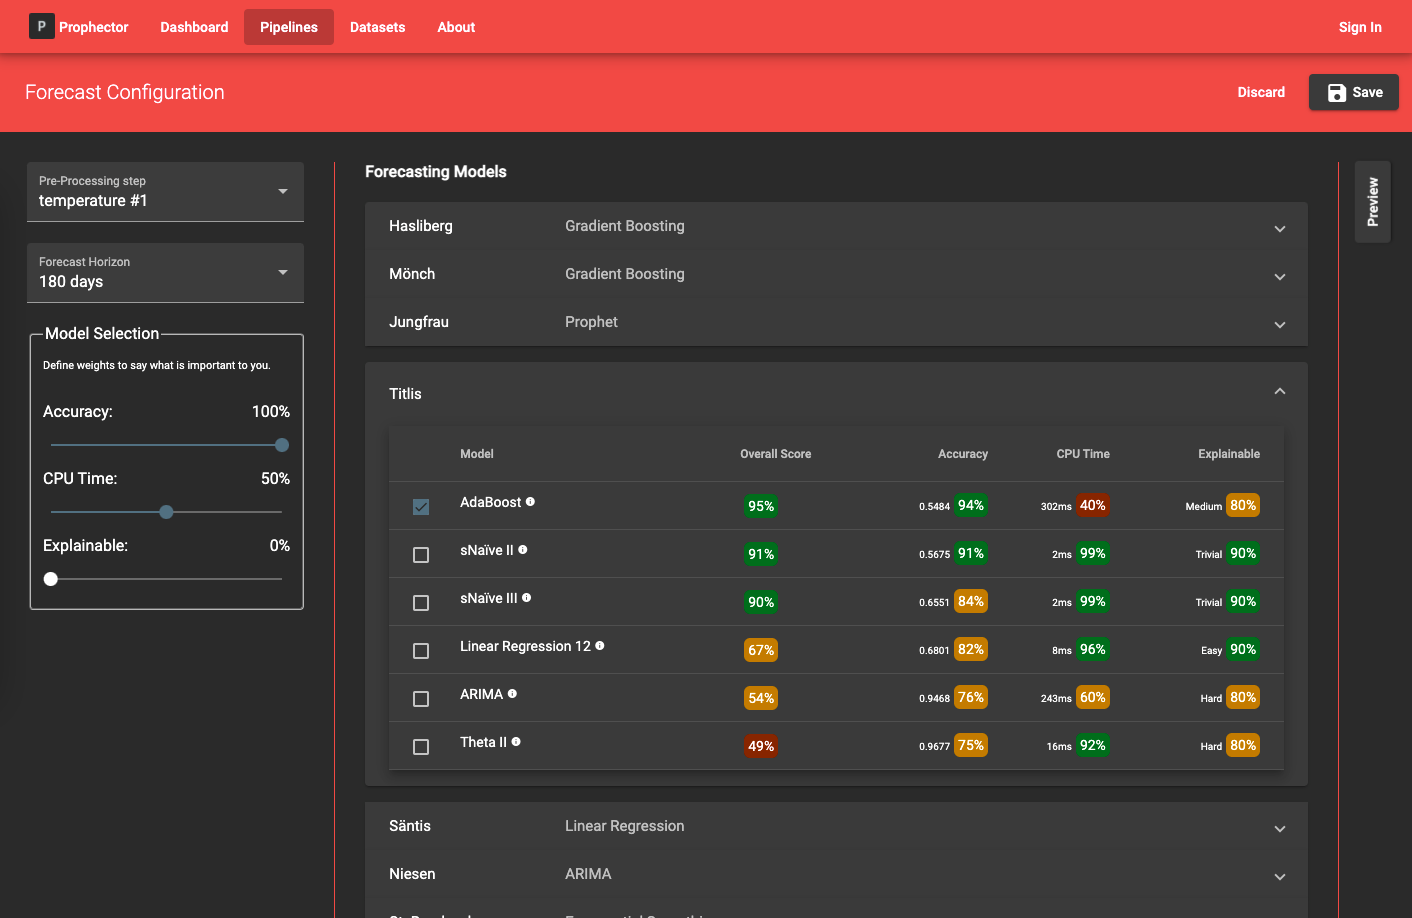
\includegraphics[scale=.3]{Figures/pipeline-config-screenshot.png}}
\caption{The user interface of our application lets users see the timeseries contained in their data source. First they configure sourcing, parsing and pre-processing. Then they reach this screen. Users can change or add multiple pre-processing steps. Based on their forecast horizon and weight sliders, the recommended models change. Each timeseries is presented with a list of possible models with metrics that apply for this type of timeseries. The can manually override the automatic selection. The preview button on the right allows users to inspect forecasts for the first 10 timeseries.}
\label{fig:pipeline-config-screenshot}
\end{figure*}

\subsection{Forecast Analysis}

After the user has configured a pipeline, they can search for timeseries within their dataset. Navigating to this timeseries then reveals the sourced data, the forecast and optionally the anomalies annotated on the graph.

Alongside are meta information such as when this data was fetched, when it was forecasted, the model used, the sensitivity and so forth.

The user commonly wants to act upon seeing the forecast, so it should be easily shareable by URL. If configuration changes become necessary, the in app links should point the user to the configuration of the pipeline steps. If they want to change something particular about this timeseries only, e.g., they want to adjust the anomaly sensitivity for that timeseries, they can do so right there without having to leave the screen..


\section{Evaluation}

In this section we will evaluate our Guided Model selection approach by comparing the results with leaderboards of two forecasting competitions.


\subsection{M5 Forecast Accuracy Competition Results}


\begin{table}
\fontsize{9pt}{12pt}\selectfont
\begin{tabular}{rlllll|lp{5cm}}
\#      & $fh$ & Freq. & $sp$ & Strictly pos. & Window       & Model & Parameters \\
\hline
 27,616 &  28  & D     & 1    & no            & [4y,   100y) & Linear Regr. & deg: 1, deseasonal mod.: additive, fit intercept: yes, normalize: no, window: 56 \\
 13,191 &  28  & D     & 1    & no            & [480d, 4y)   & Linear Regr. & deg: 1, deseasonal mod.: additive, fit intercept: yes, normalize: no, window: 28 \\
 10,562 &  28  & D     & 7    & no            & [4y,   100y) & sNa\"ive     & sp: 7, strategy: mean, window: 112 \\
  7,976 &  28  & D     & 7    & no            & [480d, 4y)   & sNa\"ive     & sp: 7, strategy: mean, window: 112 \\
  1,107 &  28  & D     & 1    & no            & [180d, 480d) & Theta        & deseasonalize: no \\
    450 &  28  & D     & 7    & no            & [180d, 480d) & sNa\"ive     & sp: 7, strategy: mean, window: 28 \\     
     78 &  28  & D     & 1    & no            & [56d,  180d) & Theta        & deseasonalize: no
\end{tabular}
\caption{M5 competition: The evaluated models to be used per group of timeseries. The first column shows how many timeseries are in that group. Our approach seems to have chosen sNa\"ive for all timeseries that contain a weekly seasonality and Theta and Linear Regression for timeseries without seasonality. We also see that Theta is favored if the training window is shorter, vs Linear Regression that seems to perform better with longer windows.}
\label{tab:m5GroupsAndModels}
\end{table}


With our guided model selection approach and the gathered configuration summaries we can determine which models should work best for a new problem. To verify our approach, we tested it by running it for the M5 forecast competition dataset. We did not use the M5 dataset in our training, so we do not create a bias towards it. However, we have collected datasets that are similar in terms of sparsity, amplitude, length, and so forth. We particularly also had a sales data set from another competition in place besides others. So, there is a slight bias towards this kind of data in our training set.


\begin{figure*}
\centerline{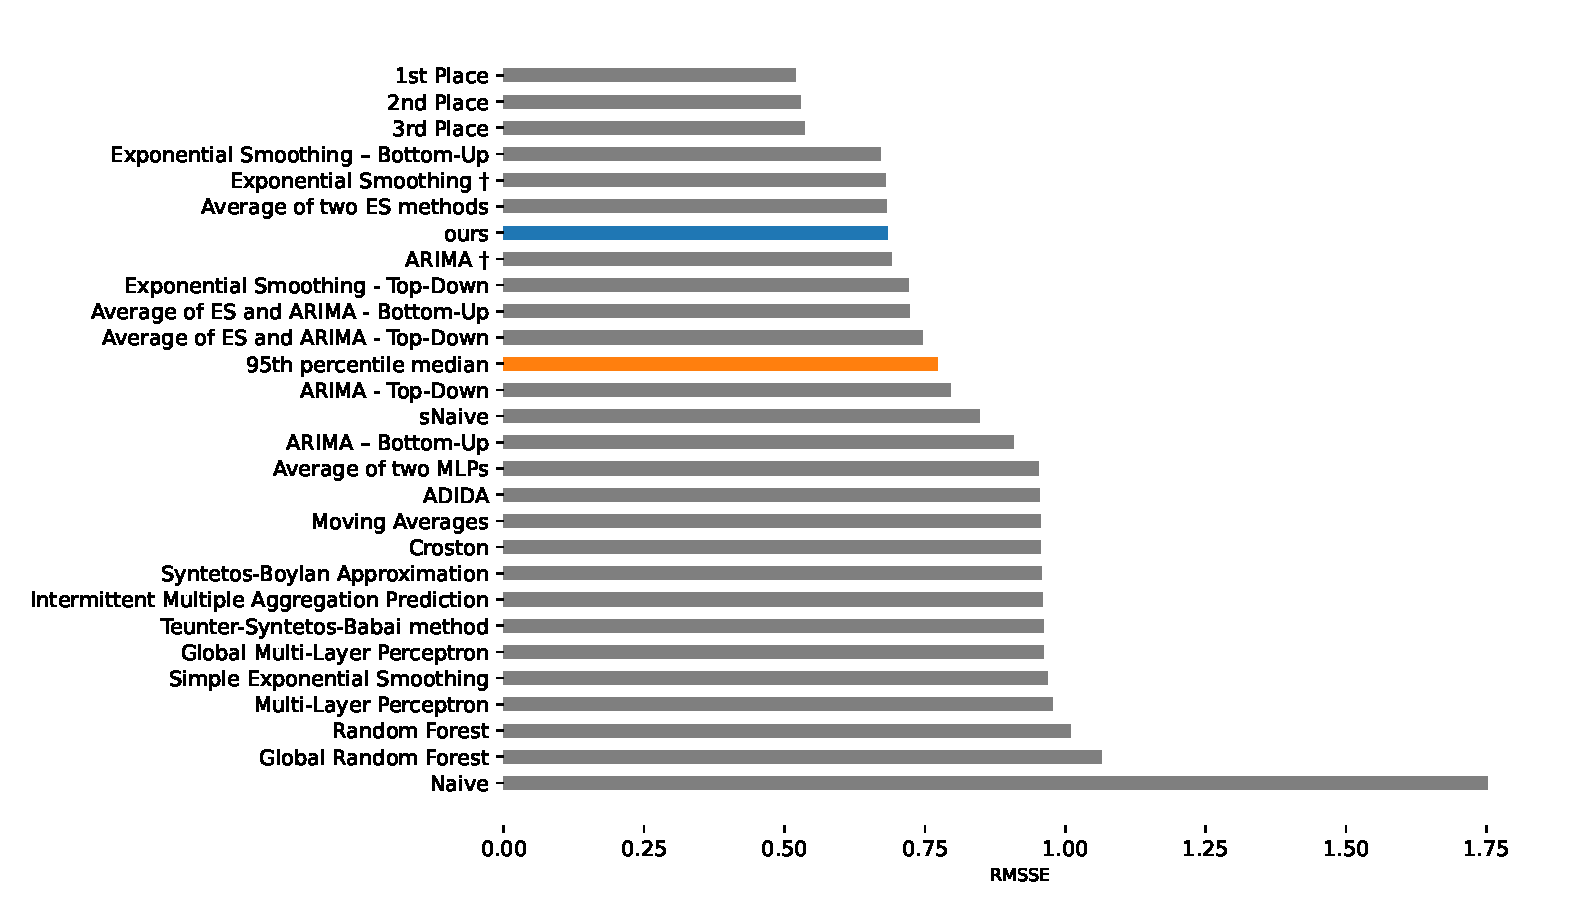
\includegraphics[scale=.6]{Figures/m5-leaderboard.eps}}
\caption{M5 Competition: The comparison of RMSSE scores with the top three places, ours and a series of baselines. \textdagger Model with explanatory (exogenous) variables. The 95\textsuperscript{th} percentile median is computed over all scores. We first took the percentile value and then built the median of all scores below that. Submitting forecasts with all zeros would result in a RMSSE score of 5.39065.}
\label{fig:m5-leaderboard}
\end{figure*}

First, we created the timeseries groups of the 30,490 M5 timeseries. This gave us the following set of groups and the best model for it. We only regard the accuracy metric as important for this competition, so we set the weights for CPU time and explainability to zero. See table \ref{tab:m5GroupsAndModels} for the elected models per group. The final submission is a combination of both validation and evaluation timeseries, which is why the total number of timeseries per group is doubled in this table.

We then created forecasts with those models and uploaded it to Kaggle. On Kaggle there usually are two leaderboards. For the M5 competition the public leaderboard is based on validation data that has been provided during the competition timeframe. Thus, it is possible to cheat and use the provided data to train a forecaster. The private leaderboard is based on hidden test data and each forecast's RMSSE score is weighted per timeseries with unknown weights. The leaderboards are calculated with approximately 50\% of the test data. Figure \ref{fig:m5-leaderboard} shows the leaderboard with the top three participants, our approach and a series of benchmarks. The benchmark scores are based on the results published by the hosts of the M5 competition. We have reproduced the Na\"ive and sNa\"ive scores and ended up with numerically almost the same scores.

Our approach resulted in a RMSSE score of 0.68382. This score is in the top 8.8\% of all submissions. We find that score to be competitive as only one single model benchmark had a lower error term. We would not expect to have a significantly lower error than the best benchmarks since we are only using benchmark models ourselves, although in a combined fashion. We also computed the forecast in less time than most of those benchmark models take by themselves since we had 31\% of our timeseries forecasted with sNa\"ive, a method that takes roughly 8ms to create a forecast. Linear Regression takes roughly 66ms and Theta 14ms. The total CPU time to compute the forecasts for the 60,980 timeseries was roughly 47 minutes. With multiprocessing on a machine with 8 cores, it took around 6 minutes (on a Macbook Pro, 2.6 GHz 6-Core Intel Core i7).

Although we do not know the times it took the competition hosts to compute the benchmark results, we argue that this ratio of accuracy and CPU time is hard to beat all the while did not even consider CPU time while selecting the models.

\subsection{Web Traffic Forecast Competition Results}

The Web Traffic Forecast competition requires participants to compute a 65-day forecast on roughly 145,000 timeseries. The forecast accuracy is measured in sMAPE, which is not ideal as we discussed earlier. The Web Traffic data is different from the M5 data in the sense that it contains a lot of strictly positive timeseries with high traffic values. We do not have a large amount of similar data in our datasets that we used to evaluate models. Specifically, we encountered that the largest group in the Web Traffic dataset had no equivalent dataset in our library to pick an evaluated model from. We used a fallback of sNa\"ive with strategy \emph{mean}. The groups designed to be generic also do not contain a forecasting horizon of 65 days. We took the closest value of 60 which likely had a small negative on finding the best models. The groups and mapped models can be seen in table \ref{tab:webTrafficGroupsAndModels}. Altogether, this proved to be not successful at all since our resulting sMAPE score was 61.08807. Our benchmarks for Na\"ive and sNa\"ive scored 49.26081 and 47.62652 respectively. The first three places reached scores of 35.48, 36.78 and 36.85. We find that valid and varied datasets are required to assume a well-fitting model can be recommended. Our models performed worse than a baseline method. We think this can also be attributed to the selection of Gradient Boosting which was chosen because of a bias towards less flaky data in our datasets than the web traffic data has.

We think we could improve this if we collect enough data and rerun our evaluation.

\begin{table}
\fontsize{9pt}{12pt}\selectfont
\begin{tabular}{rlllll|lp{5cm}}
\#      & $fh$ & Freq. & $sp$ & Strictly pos. & Window       & Model                & Parameters \\
\hline
 48,518 &  60  & D     & 7    & yes           & [480d,   4y) & Fallback to sNa\"ive & sp: 7, strategy: mean \\
 48.191 &  60  & D     & 1    & yes           & [480d,   4y) & Linear Regr.         & deg: 1, deseasonal mod.: add, fit~intercept: yes, normalize: yes, window: 60 \\
 42,460 &  60  & D     & 1    & no            & [480d,   4y) & Gradient Boosting    & deg: 1, deseasonal mod.: add, learn.~rate: 0.1, max~depth: 3, max~feat.: auto, n~estimators: 100, subsample: 1, sp: 1 \\
  5,892 &  60  & D     & 7    & no            & [480d,   4y) & Fallback to sNa\"ive & sp: 7, strategy: mean \\
      1 &  60  & D     & 1    & no            & [180d, 480d) & Theta                & deseasonalize: no \\
      1 &  60  & D     & 1    & no            & [0,     56d) & Fallback to sNa\"ive & sp: 7, strategy: mean \\
\end{tabular}
\caption{Web Traffic Competition: The evaluated models to be used per group of timeseries. Our missing data that contains weekly seasonality and is strictly positive required us to fallback to a baseline method for the biggest group.}
\label{tab:webTrafficGroupsAndModels}
\end{table}


\newpage
\section{Conclusion}
In this work we had to goal to provide an approach to guide model selection for forecasting and anomaly detection in a scalable manner. We additionally showcased how a system like this can be built in practice.

Firstly, we explored if we could classify timeseries data to predict which model will work best solely on the previous evaluation against a series of models. We concluded that this Auto Selection approach does not work if the dataset and the learning task are too similar. The evaluated classifiers were not able to learn the classes even with a very reduced number of classes. We tried classical feature extraction and Random Forests, ROCKET, MrSEQL and others to classify the timeseries without success. We discovered however that there are some timeseries which can be separated in such a space.

Thus, we followed suit with our second approach that we called Guided Model Selection. We defined groups for timeseries to fall into based on simple and few criteria. We then evaluated again a series of models against those groups and recorded the scores and timings in summaries. We then took unseen data, sorted it to fall into the groups and created forecasts with the best model according to our previous evaluation. We found that our approach can produce decent forecasts in the M5 competition. We reason that this is because the dataset used to evaluate had similar data to the M5 dataset. Our second verification using the Web Traffic dataset failed as we did not have enough data to evaluate our models against. Thus, we had to fallback to default models, which create a worse score than a baseline method. 

This guided approach is helpful for users who want to learn what models they could try to create forecasts. It gives them insights how models performed on similar data since they were evaluated on the same group. Users can inspect accuracy, CPU time and explainability and adjust weights to create their personalized ranking of models.

Our implementation and its architecture also showcase that building such a system in a highly scalable fashion can be done. We show that with modern technologies and by leveraging hyper-scalers we can build it on a pay-as-you-go model, meaning if there are no users, there are no bills. By putting a price tag on the CPU time in our system while the user is selecting a model, might lead them to tradeoff between accuracy and cost. Our scoring formula gives them the freedom to do so.



\newpage
\section{References}
\bibliographystyle{IEEEbib}
\bibliography{refs}


\end{document}
